%%%%%%%% ICML 2025 EXAMPLE LATEX SUBMISSION FILE %%%%%%%%%%%%%%%%%

\documentclass{article}

% Recommended, but optional, packages for figures and better typesetting:
\PassOptionsToPackage{table}{xcolor}
\usepackage{xcolor} 

\usepackage{microtype}
\usepackage{graphicx}
\usepackage{subfigure}
\usepackage{tcolorbox} % Load after xcolor
\usepackage{multirow}
\usepackage{comment}
\usepackage{enumitem}
\usepackage[utf8]{inputenc}
\usepackage[T1]{fontenc}  
\usepackage{lmodern} 
\usepackage{amsmath}
%\usepackage[hyphens]{url}
%\usepackage{hyperref}  
\usepackage[hyphens]{url}
\usepackage{hyperref}
\usepackage[hyphenbreaks]{breakurl}

\usepackage{xurl} % Automatically break URLs
% \usepackage[breaklinks]{hyperref} % Allow hyperlinks to break


\usepackage{tipa}
\usepackage{tikz} % Load after xcolor
\usetikzlibrary{arrows}
\usetikzlibrary{shapes.geometric, positioning, fit}
\usepackage{endnotes}


%\let\footnote=\endnote

% hyperref makes hyperlinks in the resulting PDF.
% If your build breaks (sometimes temporarily if a hyperlink spans a page)
% please comment out the following usepackage line and replace
% \usepackage{icml2025} with \usepackage[nohyperref]{icml2025} above.
\usepackage{hyperref}


% Attempt to make hyperref and algorithmic work together better:
\newcommand{\theHalgorithm}{\arabic{algorithm}}

% Use the following line for the initial blind version submitted for review:
% \usepackage{icml2025}

% If accepted, instead use the following line for the camera-ready submission:
\usepackage[accepted]{icml2025}

% For theorems and such
\usepackage{amsmath}
\usepackage{amssymb}
\usepackage{mathtools}
\usepackage{amsthm}

% if you use cleveref..
\usepackage[capitalize,noabbrev]{cleveref}

%%%%%%%%%%%%%%%%%%%%%%%%%%%%%%%%
% THEOREMS
%%%%%%%%%%%%%%%%%%%%%%%%%%%%%%%%
\theoremstyle{plain}
\newtheorem{theorem}{Theorem}[section]
\newtheorem{proposition}[theorem]{Proposition}
\newtheorem{lemma}[theorem]{Lemma}
\newtheorem{corollary}[theorem]{Corollary}
\theoremstyle{definition}
\newtheorem{definition}[theorem]{Definition}
\newtheorem{assumption}[theorem]{Assumption}
\theoremstyle{remark}
\newtheorem{remark}[theorem]{Remark}

% Todonotes is useful during development; simply uncomment the next line
%    and comment out the line below the next line to turn off comments
%\usepackage[disable,textsize=tiny]{todonotes}
\usepackage[textsize=tiny]{todonotes}


% The \icmltitle you define below is probably too long as a header.
% Therefore, a short form for the running title is supplied here:
\icmltitlerunning{}

\begin{document}

\twocolumn[
\icmltitle{Bridge the Gaps between Machine Unlearning and AI Regulation}

% It is OKAY to include author information, even for blind
% submissions: the style file will automatically remove it for you
% unless you've provided the [accepted] option to the icml2025
% package.

% List of affiliations: The first argument should be a (short)
% identifier you will use later to specify author affiliations
% Academic affiliations should list Department, University, City, Region, Country
% Industry affiliations should list Company, City, Region, Country

% You can specify symbols, otherwise they are numbered in order.
% Ideally, you should not use this facility. Affiliations will be numbered
% in order of appearance and this is the preferred way.
\icmlsetsymbol{equal}{*}

\begin{icmlauthorlist}
\icmlauthor{Bill Marino}{equal,yyy}
\icmlauthor{Meghdad Kurmanji}{equal,yyy}
\icmlauthor{Nicholas D. Lane}{yyy}
% \icmlauthor{Firstname3 Lastname3}{comp}
% \icmlauthor{Firstname4 Lastname4}{sch}
% \icmlauthor{Firstname5 Lastname5}{yyy}
% \icmlauthor{Firstname6 Lastname6}{sch,yyy,comp}
% \icmlauthor{Firstname7 Lastname7}{comp}
%\icmlauthor{}{sch}
% \icmlauthor{Firstname8 Lastname8}{sch}
% \icmlauthor{Firstname8 Lastname8}{yyy,comp}
%\icmlauthor{}{sch}
%\icmlauthor{}{sch}
\end{icmlauthorlist}

\icmlaffiliation{yyy}{Department of Computer Science and Technology, University of Cambridge, Cambridge, UK}
% \icmlaffiliation{comp}{Company Name, Location, Country}
% \icmlaffiliation{sch}{School of ZZZ, Institute of WWW, Location, Country}

\icmlcorrespondingauthor{Bill Marino}{wlm27@cam.ac.uk}
% \icmlcorrespondingauthor{Firstname2 Lastname2}{first2.last2@www.uk}

% You may provide any keywords that you
% find helpful for describing your paper; these are used to populate
% the "keywords" metadata in the PDF but will not be shown in the document
\icmlkeywords{Machine Learning, ICML}

\vskip 0.3in
]

% this must go after the closing bracket ] following \twocolumn[ ...

% This command actually creates the footnote in the first column
% listing the affiliations and the copyright notice.
% The command takes one argument, which is text to display at the start of the footnote.
% The \icmlEqualContribution command is standard text for equal contribution.
% Remove it (just {}) if you do not need this facility.

%\printAffiliationsAndNotice{}  % leave blank if no need to mention equal contribution
\printAffiliationsAndNotice{\icmlEqualContribution} % otherwise use the standard text.

\begin{abstract}
\begin{abstract}
Retrieval-Augmented Generation (RAG) is often used with Large Language Models (LLMs) to infuse domain knowledge or user-specific information. In RAG, given a user query, a retriever extracts chunks of relevant text from a knowledge base. These chunks are sent to an LLM as part of the input prompt. Typically, any given chunk is repeatedly retrieved across user questions. However, currently, for every question, attention-layers in LLMs fully compute the key values (KVs) repeatedly for the input chunks, as state-of-the-art methods cannot reuse KV-caches when chunks appear at arbitrary locations with arbitrary contexts. Naive reuse leads to output quality degradation.  This leads to potentially redundant computations on expensive GPUs and increases latency. In this work, we propose \sys, a system for managing and reusing precomputed KVs corresponding to the text chunks (we call \textit{chunk-caches}) in RAG-based systems. We present how to identify \hl{\textit{chunk-caches} that are reusable}, how to efficiently perform a small fraction of recomputation to \textit{fix} the cache to maintain output quality, and how to efficiently store and evict \textit{chunk-caches} in the hardware for maximizing reuse while masking any overheads. With real production workloads as well as synthetic datasets, we show that \sys reduces redundant computation by \textbf{51\%} over SOTA prefix-caching and \textbf{75\%} over full recomputation.
\hl{Additionally, with continuous batching on a real production workload, we get a \textbf{1.6$\times$} speedup in throughput and a \textbf{2$\times$} reduction in end-to-end response latency over prefix-caching while maintaining quality, for both the \llama-3-8B and \llama-3-70B models. 
}
\end{abstract}





\end{abstract}

\section{Introduction}
\label{introduction}
\documentclass[../main.tex]{subfiles}
\graphicspath{{../images/}}
\makeatletter
\def\input@path{{../images/}}
\makeatother
\begin{document}
\section{Introduction}
\begin{figure}
\centering
\begin{tikzpicture}
\node[inner sep=0pt] (ws) at (0, 0) {
\includegraphics[height=.4\textwidth, trim={10cm 0 10cm 0},clip]{world_space.png}};
\node[inner sep=0pt] (cs) at (6,0) {\includegraphics[height=.4\textwidth, trim={10cm 1cm 10cm 4cm},clip]{conf_space.png}};
\end{tikzpicture}
\vspace{-5pt}
\label{fig:pbrm_intro}
\caption{\textbf{Left}: Shows world space obstacles as grey spheres. Robots start and goal configuration is colored red and green, respectively. Configurations along the computed path are colored transparent blue. \textbf{Right:} Mapped world space scenario to configuration space. Obstacle region is the grey mesh. Red spheres are collision-free regions computed by the neural SCDF. The optimized shortest path in the convex corridor is the blue curve.}
\vspace{-25pt}
\end{figure}
Motion planning is the problem of finding a collision-free trajectory that connects a given start and goal configuration. The planning takes place in the configuration space of the robot. For single body robots, like mobile robots or drones, the configuration space and the world space are usually the same. This simplifies the planning, since explicit obstacle representations are available which enables geometrical tools like separating hyperplanes, smallest distance to obstacles etc., to be used when designing motion planning algorithms. For multi-body robots like manipulators, the situation is completely different. The world space obstacles are usually mapped to non-convex regions, and to make the problem even harder, the mapping is usually not known. Forming explicit representations of the obstacle region in the configuration space is usually too expensive or intractable. Despite all of this, sampling based planners are used with great success, which mainly is due to their use of implicit representations of the obstacle region. The basic idea is to construct a graph in the configuration space that covers and connects the collision-free region. From this graph, a path can be extracted that connects a given start and goal configuration. The approach is computationally expensive, since the graph is constructed with the smallest geometrical building block available, points, which represents a collision-check. Furthermore, the extracted paths from the graph are non-smooth and jagged due to the stochastic nature of the approach. This adds an additional post-processing step to the process, where the paths are shortcutted and smoothened, before the path can be used for tracking. Clearly a lot of time is invested to form this graph and produce smooth paths. Thus, if the obstacles start to move, then all of this work is done in no use, since all points that make up this graph need to be re-verified, which is simply too time consuming to be done in real time.
\\\\
In this work, we want to address the existing drawbacks of the sampling based planners. Our main contribution is an improved motion planner where each vertex in the graph covers a collision-free region in the form of a sphere instead of a point and where the edges are formed with neighboring intersecting spheres. This representation has the advantage of instead of returning piecewise linear paths, returning a sequence of overlapping spheres, i.e. a convex corridor, that connects a given start and goal configuration, illustrated in Figure \ref{fig:pbrm_intro}. This convex corridor allows us to use convex optimization to produce smooth trajectories, instead of computationally expensive post-processing methods. The representation further allows us to estimate the coverage of the collision-free space, which gives us awareness and feedback in the offline roadmap construction phase. Finally, our representation is simple to adapt to moving obstacles, simply requery for the new radii and recheck for intersections. 
\\\\
The spherical collision-free regions are formed using a signed distance function (SDF), which is a function that returns the smallest distance from an arbitrary point to the boundary of an obstacle. As the name implies, the distance is signed, thus if the point is inside the obstacle it is negative otherwise positive. If the distance is positive, a sphere with radius equal to the distance is guaranteed to cover a collision-free region. Using an SDF in motion planning is not new, but what is novel about our approach is that we express the distance in the configuration space instead of the world space and by doing so allows us to form these convex collision-free regions. We refer to the resulting SDF as a signed configuration distance function (SCDF). Computing an SCDF analytically is non-trivial, our approach is therefore to parameterize the SCDF with a deep neural network and learn the mapping by supervised learning. Our resulting neural SCDF can compute distances for different parameter values of obstacle shapes and we also show how multiple distances can be combined, thus making our approach flexible.
\section{Related work}
Motion planning algorithms can roughly be divided into three families, grid-based, sampling based and optimization based methods. Grid-based methods (GBM) discretize the planning space from which a graph is then compiled. A standard search method is A$^\star$ \citep{a_star}, which is classified as an \textit{informed} search method, since it employs a heuristic function to speed up the search. A$^\star$ guarantees to return an optimal path at the level of discretization used. GBMs usually discretize the planning space by a regular lattice and this limits the GBMs to problems with low dimensionality due to the curse of dimensionality. Thus, GBMs are usually limited to single-body robots where the degrees of freedom (DOF) are low. To overcome the inherent scaling problem with the GBMs, stochastic methods are usually used for multi-body robots. These methods are termed as sampling-based methods (SBM) and core members within this family are the rapidly-exploring random trees (RRT) \citep{rrt} and the probabilistic roadmap (PRM) \citep{prm}. RRT grows a tree from the start configuration and explores the collision-free region in a rapid way until it is able to connect to the goal region. RRT is usually improved by bi-directional planning \citep{rrt_connect}, i.e. an additional tree is grown from the goal configuration and the trees are tested for connection after any tree has been expanded. RRT is a single-query method, thus it searches for a path from scratch each time it is queried. Contrary to this, PRM is a multi-query method, which solves for multiple queries without starting from scratch. PRM does this by creating a roadmap (graph) that covers the collision-free space as an offline step. The graph is then used to solve for multiple queries. PRMs are used in cases where the environment does not change since the extra offline step is too computationally costly and needs to be re-done if the environment is changed. In our work, we address this inherent issue by using a different roadmap representation. Our vertices in the graph cover a collision-free region in the form of spheres and we form the edges by checking for intersecting spheres. If something in the environment changes, we recompute the spheres radii and recheck the intersections, without relying on collision detection. We use a trained neural network to compute the sphere radius, therefore querying for the radius can be done fast, hence our representation enables the PRM for dynamic environments.
\\\\
In the recent decades, optimization based methods (OBM) \citep{chomp, schulman, itomp, stomp} have been introduced as an alternative to SBM for multi-body robots. Like the SBM, the OBMs scale well to higher dimensional problems and produce smoother motion. It is common to use a SDF in the optimization since it is a smooth function, thus enabling gradient-based methods. However, the standard way of expressing the SDF is in world space. The distance therefore needs to be mapped to the configuration space by the forward kinematics. This mapping makes the optimization problem a non-linear program (NLP), which is computationally expensive to solve. Recently, a different approach has been proposed. In \cite{mp_gcs} motion planning is formulated as a convex optimization problem by using the graph of convex sets framework \citep{gcs}. The underlying idea is to decompose the collision-free space into intersecting convex sets from which a convex optimization problem is formulated. In cases where an explicit representation of the obstacles in the configuration space exists, like for single-body robots, creating collision-free convex regions can be done fast \citep{iris}. For multi-body robots, this is non-trivial. Existing work does this successfully \citep{iris_nlp, iris_c} by an optimization based approach, but the methods are still too time consuming to be used in the presence of moving obstacles. Our approach is instead to use deep learning to learn an SDF expressed in the configuration space. With this, we can query for shortest distances to the collision boundary, which allows us to expand spherical regions which are collision-free. Our approach is fast and therefore enables our suggested roadmap planner to be used in dynamic environments.
\\\\
Recent research has focused on learning collision detection \citep{fk_kernel_distance, diffco, graphdistnet} by predicting the signed distance between the robot links and the surrounding obstacles in the world space. The learned SDF is used in trajectory optimization but since the distance is expressed in the world space, the problem becomes an NLP and therefore takes a long time to solve. We take a novel approach and suggest to instead express the signed distance in the configuration space. This allows us to improve the PRM at the same time as it enables convex optimization for trajectory optimization, which runs faster and is more reliable than NLP solvers. In \cite{cspf} a learned signed distance function in the configuration space is proposed similar to our approach. However, their approach is restricted to point cloud representations, while we propose to represent the obstacles as parameterized geometric shapes, e.g. spheres. Furthermore, we also show how to use our learned SCDF to improve an existing roadmap planner.
\section{Problem formulation}
A robot is located in the world space, $\W \subset \R^3 $. The unique location of the robot is given by its configuration $\q \in \C$, where $\C$ is the configuration space. The set of points covered by the robots bodies at a certain configuration is expressed as $\B(\q) \subset \W$. The robot is surrounded by $\NrObst$ obstacles $\O = \bigcup_{i=1}^{\NrObst} \O_i$, where  $\O_i \subset \W$. The representation of the obstacle in the configuration space is the set $\C\O_i = \{\q \in \C \: |\: \B(\q) \cap \O_i \neq \emptyset \}$. The obstacle space is formed as $\Co = \bigcup_{i=1}^{\NrObst} \C \O_i$. The complement is referred to as the free space, $\Cf = \C \setminus \Co$. The path planning problem is a tuple, ($\Cf$, $\qStart$, $\qGoal$), where we want to connect a query pair, consisting of a start, $\qStart$, and goal configuration, $\qGoal$, with a geometric path, $\q(s): [0, 1] \mapsto \Cf$, such that $\q(0)=\qStart$ and $\q(1)=\qGoal$, or report correctly when such a path does not exist.
\end{document}


\section{Machine Unlearning}
\label{background}
To set the stage for our analysis, we set forth, in this section, we define and provide an overview of MU and its key concepts: 

\subsection{Formal Definition of Unlearning}
Let \( M \) be a model trained on a dataset \( D \) using a training algorithm \( A \). Here, we do not distinguish between \( M \) and its parameters, and write \( M = A(D) \). An \textbf{unlearning query} is typically identified by a set of data points to be forgotten, referred to as the \textbf{forget-set} \( D_f \), and the remaining data points called the \textbf{retain-set}, \( D_r = D \setminus D_f \). The goal of an \textbf{unlearning algorithm} \( U \) is to remove from \( M \) the influence of \( D_f \). The outcome is a new model, called the \textbf{unlearned model}, denoted as \( M_u = U(M; D_f, D_r) \). Depending on the unlearning approach, \( U \) may not have access to \( D_r \) \cite{zhao2024unlearningdifficulty}. In MU research, the notion of "removing influence" has been formalized using definitions from \textbf{differential privacy}. We borrow a version of this definition from \citep{ginart2019makingaiforget} as follows:


\textbf{Definition 2.2.1} Assume that \(U\) and \( A \) are stochastic processes. \(U\) is called an \((\epsilon, \delta)\)-unlearner if the distribution of \( A(D_r) \) and \( U(M; D_f, D_r) \) is \((\epsilon, \delta)\)-close. Specifically, two distributions \( \mu \) and \( \nu \) are \((\epsilon, \delta)\)-close if, for all measurable events \( B \), the following inequalities hold: \(\mu(B) \leq e^\epsilon \nu(B) + \delta\) and \(
\nu(B) \leq e^\epsilon \mu(B) + \delta
\).

This definition provides a natural taxonomy for MU algorithms. When \( \epsilon = \delta = 0 \), \( U \) is termed \textbf{exact unlearning}; otherwise, it is referred to as \textbf{approximate unlearning}.

\subsection{Informal Definitions}
While Def. 2.2.1 provides a rigorous mathematical formulation for MU, researchers often rely on informal interpretations, typically phrased as \texttt{removing [\dots] from $M$}. Deriving informal definitions from Def. 2.2.1 is not always straightforward. A key challenge is that the entity to be removed, may not be clearly identifiable --e.g., in generative models, \texttt{[\dots]} often corresponds to a fact or concept that lacks an explicit representation in either $M$ or $D$.

However, we contend that overly broad definitions of MU introduce unnecessary complexity, potentially hindering clear scientific discourse. In this paper we shall limit unlearning to those techniques in ML that modify the parameter-set of the model (e.g. by deleting and retraining, fine-tuning, or adding/removing some parameters). With this condition, MU still can serve as a tool--among others--for applications such as safeguarding and alignment. At the same time, it leaves methods such as guardrailing (or any "output suppression" as per \cite{cooper2024machineunlearningdoesntthink}) independent of MU, which deserve their own distinct discussion and evaluation in the context of regulations and beyond.

%For instance, recent work \cite{cooper2024machineunlearningdoesntthink} encompasses output safeguarding techniques under the umbrella of unlearning. This expansive definition can potentially complicate the development of scientifically precise and generalizable arguments about unlearning, diluting its conceptual clarity.}



\subsection{Evaluation metrics} 

While Definition 2.2.1 is widely accepted in the MU community, it presents several challenges in practical settings. First, some works question whether this definition is necessary or sufficient to achieve true MU \cite{thudi2022necessityauditing}. Second, in large-scale applications, it is computationally infeasible to directly measure the closeness between the distributions \( A(D_r) \) and \( U(M; D_f, D_r) \). As a result, researchers often resort to alternative proxies to verify MU. These proxies include performance metrics (e.g., classification accuracy \citep{golatkar2020eternal} or generative performance using metrics like ROUGE for large language models \citep{maini2024tofutaskfictitiousunlearning}) and privacy attacks, such as membership inference attacks or backdoor attacks \cite{hayes2024inexactunlearning, triantafillou2024arewemakingprogress}.


\subsection{Unlearning Axes} 
Creating a taxonomy for MU depends on the goal and perspective. Instead of suggesting a new taxonomy, here, we outline two key dimensions that help identifying a MU problem: Model Type, and Forget-Set Definition. 

\textbf{Model Type.} MU is studied in both discriminative and generative models. MU algorithms depend on the training objective and the architectures of these models. For example, \textit{Negative Gradient}, a widely used MU strategy, has different formulations in image classifiers \cite{golatkar2020eternal} versus language models \cite{yao2024muofllms}. Within these two broad categories, one can imaging further subcategories based on data type, evaluation metrics, etc. 

\textbf{Forget-Set Definition.} The forget-set, or the target of MU, can take various forms. It usually is in the following forms: a) the entire data class(es), b) individual data points \cite{kurmanji2023unboundedmachineunlearning}, c) shared features across data points \citep{warnecke2021muoflabelsfeatures}, and d) knowledge (also referred to as concepts or behaviors) that transcends direct connections to the training data \citep{gandikota2024unifiedconceptdelete}.

%\subsubsection{Application}
%MU was originally proposed as a solution for compliance with GDPR's "right to be forgotten" in ML models. Although Article 17 does not explicitly mandate the deletion of data from ML models, research in MU has extended the interpretation of the regulation to encompass such models, often without a comprehensive legal analysis. However, recent work \cite{??}, however, has critically examined MU within the framework of GDPR, concluding that only "retraining from scratch" meets the stringent requirements for compliance. Subsequently, MU has been adapted to address other regulatory and ethical challenges. For instance, it has been employed to remove biases from generative models \cite{omkar}, eliminate backdoors introduced into ML models through poisoned data \cite{?}, delete copyrighted content embedded within model training data \cite{?}, and removing outdated data \cite{?}.

\subsection{Trade-offs and risks}
MU algorithms strive to make a balance between three key objectives: \textbf{Model Utility}, \textbf{Forgetting Quality}, and \textbf{Efficiency}. In certain privacy-centric applications, forgetting can be synonymous with achieving privacy \citep{liu2024breaking}. Hyperparameters and regularizers impact these trade-offs. For example, in MU via \texttt{Fine-tune}, the number of steps and learning rate dictate the balance between forgetting quality and efficiency. Similarly, in \texttt{Gradient Ascent}, the number of steps determines the trade-off between effective MU and preserving model's utility.

Additionally, forgetting may sometimes conflict with privacy due to two phenomena. First, unlearning specific data points can inadvertently expose information about others in the retained set due to the "onion effect" of privacy \citep{carlini2022privacyonioneffectmemorization}. Second, over-forgetting \citep{kurmanji2023unboundedmachineunlearning} a data point may reveal its membership in the original training set—a phenomenon known as the "Streisand Effect" \citep{golatkar2020eternal}. Addressing these challenges requires careful calibration of MU methods to ensure a delicate equilibrium across these competing objectives. These trade-offs are illustrated in \autoref{fig:updated-tradeoffs-diagram}.

Beyond these trade-offs, MU introduces risks associated with \textit{untrusted parties} \citep{li2024pseudounlearning} and \textit{malicious unlearning} \citep{qian2023towardsmaliciousunlearning}. Malicious entities could exploit MU to make fake deletion queries, or introduce computation overheads to the system \citep{marchant2022hardtoforget}.

% \begin{figure}[h!]
%     \centering
%     \resizebox{\columnwidth}{!}{% Resize the entire TikZ picture to fit one column
%         \begin{tikzpicture}[
%             % Define styles for different elements
%             nodeStylePrimary/.style={
%                 draw, 
%                 ellipse, 
%                 text centered, 
%                 minimum height=1.5cm, 
%                 minimum width=3cm, 
%                 font=\bfseries
%             },
%             nodeStyleSecondary/.style={
%                 draw, 
%                 rectangle, 
%                 rounded corners, 
%                 text centered, 
%                 minimum height=1cm, 
%                 minimum width=2cm, 
%                 font=\bfseries
%             },
%             arrowStyleTradeoff/.style={
%                 <->, 
%                 thick, 
%                 solid, 
%                 -latex
%             },
%             arrowStylePrivacy/.style={
%                 <->, 
%                 thick, 
%                 dashed, 
%                 -latex
%             },
%             arrowStyleControl/.style={
%                 ->, 
%                 thick, 
%                 dotted, 
%                 -latex
%             },
%             legendBox/.style={
%                 draw, 
%                 rectangle, 
%                 rounded corners, 
%                 fill=white, 
%                 font=\small,
%                 inner sep=5pt
%             }
%         ]
        
%         % Primary Objectives
%         \node[nodeStylePrimary, fill=blue!30] (Utility) at (0, 0) {Model Utility};
%         \node[nodeStylePrimary, fill=green!30] (Forgetting) at (4, 0) {Forgetting Quality};
%         \node[nodeStylePrimary, fill=orange!30] (Efficiency) at (2, 4) {Efficiency};
        
%         % Privacy as external factor (shifted down slightly)
%         \node[nodeStylePrimary, fill=red!30] (Privacy) at (2, -4) {Privacy};
        
%         % Hyperparameters node (shifted slightly right)
%         \node[nodeStyleSecondary, fill=yellow!30] (Hyperparams) at (6.5, 1.75) {Hyperparameters};
        
%         % Trade-off arrows (solid) with adjusted label positions
%         \draw[arrowStyleTradeoff] (Utility) -- (Forgetting) node[pos=0.6, above] {Balance};
%         \draw[arrowStyleTradeoff] (Forgetting) -- (Efficiency) node[pos=0.6, right] {Trade-off};
%         \draw[arrowStyleTradeoff] (Efficiency) -- (Utility) node[pos=0.4, left] {Trade-off};
        
%         % Privacy relationships (dashed) with shifted labels
%         \draw[arrowStylePrivacy] (Privacy) -- (Forgetting) node[pos=0.4, left] {Conflict};
%         \draw[arrowStylePrivacy] (Privacy) -- (Utility) node[pos=0.6, right] {Impact};
        
%         % Hyperparameters relationships (dotted) with adjusted angles
%         \draw[arrowStyleControl] (Hyperparams) -- (Forgetting) node[pos=0.6, above, sloped] {Adjust};
%         \draw[arrowStyleControl] (Hyperparams) -- (Efficiency) node[pos=0.4, below, sloped] {Tune};
        
%         % Annotations for Privacy Conflicts (shifted slightly outward)
%         \node[draw, diamond, fill=gray!20, minimum size=1cm, above left=0.5cm and 0.5cm of Privacy] (Conflict1) {Info Leak};
%         \node[draw, diamond, fill=gray!20, minimum size=1cm, below left=0.5cm and 0.5cm of Privacy] (Conflict2) {Membership Reveal};
%         \draw[->, dashed] (Privacy) -- (Conflict1);
%         \draw[->, dashed] (Privacy) -- (Conflict2);
        
%         \end{tikzpicture}
%     }
%     \caption{Illustration of the trade-offs in unlearning algorithms among Model Utility, Forgetting Quality, Efficiency, and Privacy. Hyperparameters serve as control elements to navigate these trade-offs. Solid arrows represent direct trade-offs, dashed arrows indicate privacy-related relationships, and dotted arrows denote the influence of hyperparameters.}
%     \label{fig:enhanced-tradeoffs-diagram}
% \end{figure}

\begin{figure}[h!]
    \centering
    \resizebox{0.8\columnwidth}{!}{%
        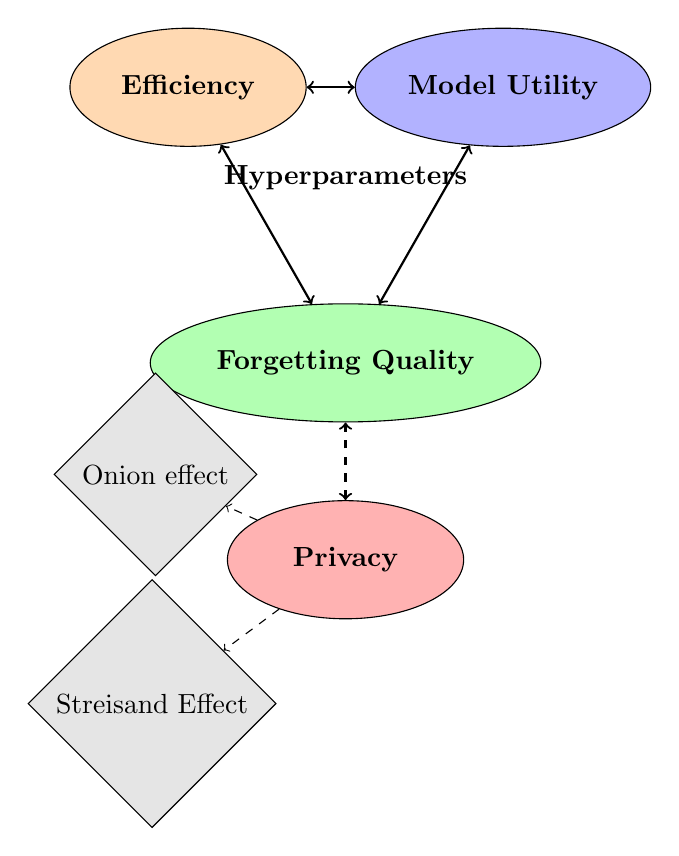
\begin{tikzpicture}[
            % Define styles for different elements
            nodeStylePrimary/.style={
                draw, 
                ellipse, 
                text centered, 
                minimum height=1.5cm, 
                minimum width=3cm, 
                font=\bfseries
            },
            arrowStyleTradeoff/.style={
                <->, 
                thick, 
                solid
            },
            arrowStylePrivacy/.style={
                <->, 
                thick, 
                dashed
            }
        ]
        
        % Repositioned Primary Objectives
        \node[nodeStylePrimary, fill=orange!30] (Efficiency) at (-2, 2) {Efficiency};
        \node[nodeStylePrimary, fill=blue!30] (Utility)    at ( 2, 2) {Model Utility};
        \node[nodeStylePrimary, fill=green!30] (Forgetting) at ( 0,-1.5) {Forgetting Quality};
        
        % Privacy below Forgetting
        \node[nodeStylePrimary, fill=red!30] (Privacy) at (0, -4) {Privacy};
        
        % Trade-off arrows among Efficiency, Utility, and Forgetting (no labels)
        \draw[arrowStyleTradeoff] (Efficiency) -- (Utility);
        \draw[arrowStyleTradeoff] (Efficiency) -- (Forgetting);
        \draw[arrowStyleTradeoff] (Utility)    -- (Forgetting);
        
        % Privacy relationship (dashed) ONLY with Forgetting (no label)
        \draw[arrowStylePrivacy] (Privacy) -- (Forgetting);
        
        % Label inside the triangle
        \node[font=\bfseries] at (0, 0.85) {Hyperparameters};
        
        % (Optional) Privacy conflict annotations (if you still want them)
        \node[draw, diamond, fill=gray!20, minimum size=1cm, above left=-0.1   cm and 0.7cm of Privacy] (Conflict1) {Onion effect};
        \node[draw, diamond, fill=gray!20, minimum size=1cm, below left=0.5cm and 0.6cm of Privacy] (Conflict2) {Streisand Effect};
        \draw[->, dashed] (Privacy) -- (Conflict1);
        \draw[->, dashed] (Privacy) -- (Conflict2);
        
        \end{tikzpicture}
    }
    \caption{\textit{\textbf{Illustration of MU trade-offs.}}}
    \label{fig:updated-tradeoffs-diagram}
\end{figure}



%MU carries several known risks and drawback which are relevant across our analysis. First, data points may be so ``embedded in the model’s implicit knowledge graph'' that it may not be possible to unlearn them without paying a price in model utility \citep{liu_unlearning_2023}. What is more, removing some data points --- e.g., to guard them from confidentiality attacks --- may increase the risk of other data points to the same attacks \citep{carlini2022privacyonioneffectmemorization}.

%\begin{figure}[h!]
\centering
\resizebox{\columnwidth}{!}{ % Resizes the figure to fit the column width
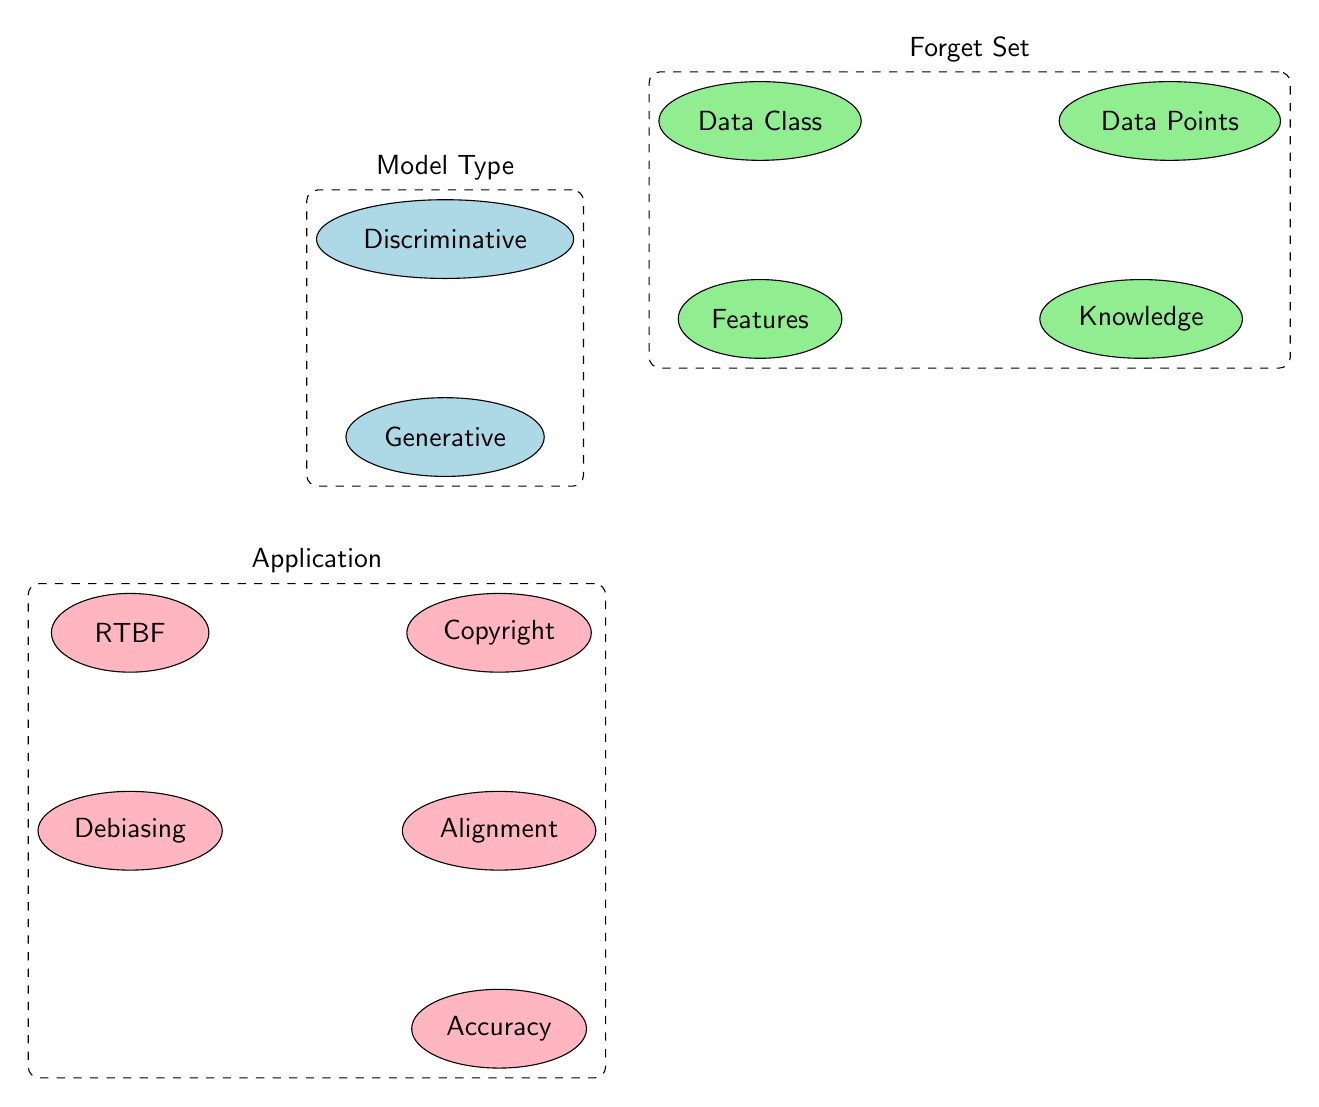
\begin{tikzpicture}[
    every node/.style={font=\sffamily},
    concept/.style={ellipse, draw, text centered, minimum width=2cm, minimum height=1cm},
    group/.style={draw, rounded corners, dashed, inner sep=5mm}
]

% Colors
\definecolor{modelColor}{RGB}{173, 216, 230} % Light Blue
\definecolor{forgetColor}{RGB}{144, 238, 144} % Light Green
\definecolor{applicationColor}{RGB}{255, 182, 193} % Light Pink

% Model Type Group
\node[concept, fill=modelColor] (discriminative) at (0, 0) {Discriminative};
\node[concept, fill=modelColor] (generative) [below=1.5cm of discriminative] {Generative};
\node[draw, rounded corners, dashed, fit={(discriminative) (generative)}, label={above:Model Type}] (modelType) {};

% Forget Set Group
\node[concept, fill=forgetColor] (dataClass) at (4, 1.5) {Data Class};
\node[concept, fill=forgetColor] (dataPoints) [right=2.5cm of dataClass] {Data Points};
\node[concept, fill=forgetColor] (features) [below=1.5cm of dataClass] {Features};
\node[concept, fill=forgetColor] (knowledge) [right=2.5cm of features] {Knowledge};
\node[draw, rounded corners, dashed, fit={(dataClass) (dataPoints) (features) (knowledge)}, label={above:Forget Set}] (forgetSet) {};

% Application Group
\node[concept, fill=applicationColor] (rtbf) at (-4, -5) {RTBF};
\node[concept, fill=applicationColor] (copyright) [right=2.5cm of rtbf] {Copyright};
\node[concept, fill=applicationColor] (debiasing) [below=1.5cm of rtbf] {Debiasing};
\node[concept, fill=applicationColor] (alignment) [below=1.5cm of copyright] {Alignment};
\node[concept, fill=applicationColor] (accuracy) [below=1.5cm of alignment] {Accuracy};
\node[draw, rounded corners, dashed, fit={(rtbf) (copyright) (debiasing) (alignment) (accuracy)}, label={above:Application}] (application) {};

\end{tikzpicture}
} % End of resizebox
\caption{Unlearning dimensions: Model Types, Forget Set, and Applications}
\label{fig:unlearning_dimensions}
\end{figure}


%AI systems developers may be using open-source models without access to the underlying training data \cite{Schneier2024}, meaning that training from scratch is not an option. Even when it is, especially for the models trained on large-scale datasets --- a category that includes many of the most powerful models today -- training from scratch can be "prohibitively costly." \cite{wu2024unlearningconceptsdiffusionmodel,cheng2023gnndeletegeneralstrategyunlearning}.


\section{The EU’s Artificial Intelligence Act}
\label{euaia}
The AIA sets forth harmonized requirements for AI systems and models placed on the market or put into service in the EU \citep[Art. 1]{european_union_ai_act_2024}. These requirements largely target two distinct categories of AI: AI systems and general-purpose AI (``GPAI'') models. Here, we define these two categories and, for each, briefly preview the requirements that, we later argue, MU may assist compliance with.
% Lastly, we outline the relationship between the AIA and GDPR, which also has a bearing on our analysis.

% Its requirements display some particular characteristics and patterns that are worth highlighting because they influence the ways MU could hypothetical be used to aid compliance with the Act.

\subsection{AI Systems}

The AIA broadly defines AI systems to include any ``machine-based system that is designed to operate with varying levels of autonomy and that may exhibit adaptiveness after deployment, and that, for explicit or implicit objectives, infers, from the input it receives, how to generate outputs such as predictions, content, recommendations, or decisions that can influence physical or virtual environments'' \citep[Art. 3.1]{european_union_ai_act_2024}. An example of a system that might meet this criteria is ChatGPT \citep{fernandez-llorca_interdisciplinary_2024}. 

In laying out its rules for these AI systems, the AIA relies on a ``risk-based'' approach \citep{Mahler2022-gc}, by which an AI system's perceived degree of risk determines the exact rules that apply to it. Here, the strictest requirements --- and the ones most relevant to our discussion --- are reserved for those AI systems deemed to be \textit{high-risk} \citep[Art. 6]{european_union_ai_act_2024}. 
% Whether or not an AI system is high-risk is largely based on its intended use \citep{edwards_eu_ai_2022}: specifically, whether the intended use falls into one of the high-risk applications enumerated by the AIA, which include critical infrastructure, education, and more \citep[Art. 6.2; Ann. III]{european_union_ai_act_2024}. 
Such high-risk AI (``HRAI'') systems are subject to a bevy of requirements \citep[Chap. III]{european_union_ai_act_2024}. Among them, the following are the most relevant to our position:\footnote{One set of AIA requirements that we have consciously excluded from our analysis is those around data and data governance for HRAI systems \citep[Art. 10]{european_union_ai_act_2024}. Our interpretation is that these requirements must be met at the dataset level and that no amount of MU on the downstream model will cure violations of these requirements. Ideally, lawmakers or courts will clarify whether our stance is the right one. If it is, then a follow-on question is whether AI system providers who repair Article 10 violations in their data are still obligated to remove the impact of this violative data on models that were trained with it. This question, of course, echoes questions around models trained on datasets that violate GDPR  \citep{JULIUSSEN2023105885, DBLP:conf/sp/BourtouleCCJTZL21, yang2024machinelearningmachineunlearning}. If the answer is in the affirmative, then MU may offer a computational efficient method for doing so --- at least as compared to retraining from scratch. \label{footnote2}}

% HRAI systems must subject their training, evaluation, and test sets (collectively, ``datasets'')  to data governance and management practices appropriate for their intended purpose \citep[Art. 10.2]{european_union_ai_act_2024}. These practices must include measures to detect, prevent and mitigate any ``possible biases that are likely to affect the health and safety of persons, have a negative impact on fundamental rights or lead to discrimination prohibited under Union law'' \citep[Art. 10.2(f-g)]{european_union_ai_act_2024}. These practices must also ``address[]'' any relevant data gaps or shortcomings that prevent compliance with other AIA provisions \citep[Art. 10.2(h)]{european_union_ai_act_2024}. Data governance and management practices aside, datasets must be ``relevant, sufficiently representative, and to the best extent possible, free of errors and complete in view of the intended purpose'' and must display ``appropriate statistical properties'' including as regards the persons or groups of persons in relation to whom the AI system is intended to be used \citep[Art. 10.3]{european_union_ai_act_2024}. The latter, states the AIA's Recitals, necessitates ``the mitigation of possible biases in the data sets'' \citep[Rec. 67]{european_union_ai_act_2024}. Lastly, datasets must ``take into account, to the extent required by the intended purpose, the characteristics or elements that are particular to the specific geographical, contextual, behavioural or functional setting within which the ... AI system is intended to be used'' \citep[Art. 10.4]{european_union_ai_act_2024}.} 


\textbf{Risk management}:
HRAI systems must implement risk management systems that include the identification of known and reasonably foreseeable risks that the system can pose to health and safety or to fundamental rights \citep[Art. 9.2(a)]{european_union_ai_act_2024, kaminski_law_review_2023}. Here, risks to \textit{health and safety}, may include risks to mental and social well-being as well as physical safety. \citep{armstrong_ai_safety_2024, european_commission_ai_qa_2021}. Meanwhile, risks to \textit{fundamental rights} includes risks to any of the rights listed on the EU's Charter of Fundamental Rights \citep{eu_charter_2000}; though, here we only focus on risks to the right most relevant to the topic of MU: the right to non-discrimination, including from biased results \citep{arnold_how_2024}.\footnote{Another fundamental right which some HRAI systems may pose risks to --- risks that must then be managed under \citep[Art. 9]{european_union_ai_act_2024} --- is the right to protection of personal data \citep[Art. 8]{eu_charter_2000}. This includes the right for personal data to ``be processed fairly'' \citep[Art. 8(2)]{eu_charter_2000}, with GDPR subsequently setting the standards for doing so \citep{european_union_gdpr_2016}. Because the application of MU to assist GDRP compliance has been extensively covered by earlier literature \citep{JULIUSSEN2023105885,yang2024machinelearningmachineunlearning} and because our focus is on the \textit{new} use cases for MU brought about by AI regulation, we do not cover it here.}
% As was the case with risks to health and safety, we posit that 
% risks to these two fundamental rights will often stem from problems in the data that MU can, in the downstream model, ostensibly repair. For example, the right to the protection of personal data protects any information relating to an identified or identifiable natural (living) person, including names, dates of birth, photographs, video footage, email addresses, telephone numbers, IP addresses and communications content \citep{edps_dataprotection}. 
Importantly, wherever these risks are identified and can be ``reasonably mitigated or eliminated through the development or design'' of the AI system \citep[Art. 9.3]{european_union_ai_act_2024}, the risk management system must address them with ``appropriate and targeted risk management measures'' \citep[Art. 9.2(d)]{european_union_ai_act_2024}. 
% When choosing these measures, consideration may be given to ``achieving an appropriate balance'' between minimizing the risks and satisfying the AIA's other requirements \citep[Art. 9.4]{european_union_ai_act_2024}. 
These risk management measures must ensure the ``residual risk associated with each hazard, as well as the overall residual risk of the [HRAI] systems is judged to be acceptable'' \citep[Art. 9.5]{european_union_ai_act_2024} and, furthermore, ensure the ``elimination or reduction'' of the identified risks ``as far as technically feasible through adequate design and development''  \citep[Art. 9.5]{european_union_ai_act_2024}.

% \paragraph{\textbf{Data and data governance}:}
% HRAI systems must subject their training, evaluation, and test sets (collectively, ``datasets'')  to data governance and management practices appropriate for their intended purpose \citep[Art. 10.2]{european_union_ai_act_2024}. These practices must include measures to detect, prevent and mitigate any ``possible biases that are likely to affect the health and safety of persons, have a negative impact on fundamental rights or lead to discrimination prohibited under Union law'' \citep[Art. 10.2(f-g)]{european_union_ai_act_2024}. These practices must also ``address[]'' any relevant data gaps or shortcomings that prevent compliance with other AIA provisions \citep[Art. 10.2(h)]{european_union_ai_act_2024}. Data governance and management practices aside, datasets must be ``relevant, sufficiently representative, and to the best extent possible, free of errors and complete in view of the intended purpose'' and must display ``appropriate statistical properties'' including as regards the persons or groups of persons in relation to whom the AI system is intended to be used \citep[Art. 10.3]{european_union_ai_act_2024}. The latter, states the AIA's Recitals, necessitates ``the mitigation of possible biases in the data sets'' \citep[Rec. 67]{european_union_ai_act_2024}. Lastly, datasets must ``take into account, to the extent required by the intended purpose, the characteristics or elements that are particular to the specific geographical, contextual, behavioural or functional setting within which the ... AI system is intended to be used'' \citep[Art. 10.4]{european_union_ai_act_2024}.

\textbf{Accuracy and cybersecurity}: 
HRAI systems must be designed and developed so as to achieve an ``appropriate level'' of accuracy and cybersecurity \citep[Art. 15.1]{european_union_ai_act_2024}. In its Recitals, the AIA stresses that these appropriate levels are a function of the system's intended purpose as well as the SOTA \citep[Rec. 74]{european_union_ai_act_2024}. When it comes to cybersecurity, the AIA specifically requires that HRAI systems be ``resilient against attempts by unauthorised third parties to alter their use, outputs or performance by exploiting system vulnerabilities'' \citep[Art. 15(5)]{european_union_ai_act_2024} and take technical measures to ``prevent, detect, respond to, resolve and control for ... data poisoning'' as well as ``confidentiality attacks'' \citep[Art. 15.5]{european_union_ai_act_2024}.

\subsection{GPAI models}

In contrast to an AI system, a GPAI model is defined as any AI model that is ``trained with a large amount of data using self-supervision at scale, that displays significant generality and is capable of competently performing a wide range of distinct tasks regardless of the way the model is placed on the market and that can be integrated into a variety of downstream systems or applications, except AI models that are used for research, development or prototyping activities before they are placed on the market'' \citep[Art. 3.63]{european_union_ai_act_2024}. Some see this as being synonymous with ``foundation model'' \citep{ada_lovelace_foundation_models_2024}. An example of a GPAI model that might meet this criteria is GPT 3.5, the model powering ChatGPT \citep{fernandez-llorca_interdisciplinary_2024}.

In laying out its requirements for GPAI models, the AIA again uses a risk-based approach, with the strictest requirements reserved for those GPAI models deemed to carry \textit{systemic risk} \citep[Art. 55]{european_union_ai_act_2024}. This is defined as the risk of ``having a significant impact on the [EU] market due to [its] reach, or due to actual or reasonably foreseeable negative effects on public health, safety, public security, fundamental rights, or the society as a whole, that can be propagated at scale across the value chain'' \citep[Art. 2.65; Annex III]{european_union_ai_act_2024}. This status can be established through a number of proxies, including performance on benchmarks and the amount of compute used during training \citep[Art. 51]{european_union_ai_act_2024}. While the AIA itself does not further elaborate on what constitutes systemic risk, the First Draft of the General-Purpose AI Code of Practice, a companion piece to the AIA that breaks it down into more granular technical standards, proposes that it covers risks related to: (1) cyber offense; (2) chemical, biological, radiological, and nuclear (CBRN); (3) loss of control; (4) automated use of models for AI research and development; (5) persuasion and manipulation; and (6) large-scale discrimination \cite{gpai_code_2024}.

Among the AIA's requirements for GPAI models that do display systemic risk --- and those that don't --- the following are the most relevant to our analysis: 

\textbf{Copyright}: 
All GPAI model providers must ``put in place a policy to comply with Union law on copyright and related rights'' \citep[Art. 53.c]{european_union_ai_act_2024}. Among other things, this policy must respect rightsholders' requests, per \citep[Art. 4(3)]{eu_dsg_directive_2019}, to opt out of text and data mining (TDM) on their copyrighted works \citep[Rec. 105, Art. 53.c]{european_union_ai_act_2024}.\footnote{As Recital 105 of the AIA explains, any use of copyright-protected content typically requires the authorization of its rightsholder \citep[Rec. 105]{european_union_ai_act_2024}. While Directive (EU) 2019/790 introduced an exception to this rule for text and data mining, it also granted rightsholders the power to opt out of the exception (unless the text and data mining is done for the purposes of scientific research) \citep[Art. 4]{eu_dsg_directive_2019}. Where the rightsholders opt out, says the AIA, providers of GPAI models must obtain an authorization from rightsholders to carry out text and data mining over their works \citep[Rec. 105]{european_union_ai_act_2024}.}

\textbf{Systemic risk}:
Those GPAI models that display systemic risk are required to ``mitigate'' it \citep[Art. 55(a-b)]{european_union_ai_act_2024}

\textbf{Cybersecurity}: 
GPAI models with systemic risk are additionally required to ``ensure an adequate level of cybersecurity'' \citep[Art. 55(d)]{european_union_ai_act_2024}.



%\begin{table*}[h!]
\centering
\caption{Summary of The European Union’s Artificial Intelligence Act.}
\label{tab:summary_ai_gpai}
\resizebox{\textwidth}{!}{%
\begin{tabular}{|l|l|p{10cm}|}
\hline
\textbf{Category} & \textbf{Key Areas} & \textbf{Details} \\ \hline
\multirow{3}{*}{AI Systems} 
    & Definition & Machine-based systems with autonomy and adaptiveness. Generates outputs like predictions, recommendations, or decisions that impact environments. \\ \cline{2-3}
    & Regulation & Risk-based approach, with stricter rules for high-risk systems. High-risk applications include critical infrastructure, education, and vocational training. \\ \cline{2-3}
    & Key Requirements & 
      - \textbf{Risk Management}: Identify and mitigate risks to health, safety, and fundamental rights. Mitigate risks through appropriate design and development measures. Balance risk minimization with other compliance requirements. \\
      & & - \textbf{Data Governance}: Datasets must be relevant, representative, error-free, and contextually appropriate. Prevent biases and address data gaps or shortcomings. \\
      & & - \textbf{Accuracy and Cybersecurity}: Ensure high accuracy and resilience to threats throughout the system's lifecycle. Protect against vulnerabilities, including data and model poisoning or adversarial attacks. \\ \hline
\multirow{3}{*}{GPAI Models} 
    & Definition & General-purpose AI models trained on large datasets, capable of diverse tasks. Example: GPT-3.5. \\ \cline{2-3}
    & Regulation & Risk-based approach, with stricter rules for models posing systemic risks. Systemic risks include societal impact, public health, and large-scale discrimination. \\ \cline{2-3}
    & Key Requirements & 
      - \textbf{Copyright Compliance}: Adhere to EU copyright laws and respect text and data mining restrictions. \\
      & & - \textbf{Systemic Risk Mitigation}: Address risks like manipulation, discrimination, or public harm. \\
      & & - \textbf{Cybersecurity}: Ensure adequate protection against systemic threats, such as adversarial attacks. \\ \hline
\end{tabular}%
}

\end{table*}


\section{Related Work}
\label{RelatedWork}
\section{Related Work}
% \subsection{Vision Language Model}
% 시각장애인에서 상황을 설명할 DB가 없으니 만들었다. 그리고 이를 VLM에 튜닝했다.
\subsection{Technical approaches for assisting the visually-impaired}


\subsection{Datasets for visual instruction tuning}


\section{MU for AIA compliance: a catalog}
\label{applications}
This Section comprehensively catalogs the potential applications of MU to assist AIA compliance. 
% In creating this catalog, we make a distinction between MU for system- and model-centered requirements like those in \citep[Art. 9, 15, 53, 55]{european_union_ai_act_2024} and MU for data-centered requirements like those in \citep[Art. 10]{european_union_ai_act_2024}. 
For each, we analyze the SOTA and its ability to support the potential application, then identify any open questions the research community must resolve in order to bridge the gap between the two. 
% \subsection{MU to aid compliance with system- and model-centered AIA requirements}
 % Some AIA provisions require AI systems or GPAI models, at large, to satisfy certain criteria --- e.g., related to risk mitigation \citep[Arts. 9, 55]{european_union_ai_act_2024}, accuracy and cybersecurity \citep[Art. 15]{european_union_ai_act_2024}, or copyright law \citep[Art. 53]{european_union_ai_act_2024}. When problematic training data points (i.e., the forget set) are what is holding the system or model back from achieving these criteria, and where MU, by diminishing the impact of those data points in an already-trained model, can help the system or model achieve the decreed criteria, it seems reasonable to hypothesize that MU can be a viable tool for compliance with these particular provisions.
 % One potential snag here might involve problematic training data points that also happen to violate requirements of the AIA (notably, those of Article 10). Are all downstream models trained on those data points ``poisoned fruit'' that are irredeemably non-compliant themselves, regardless of any post-training adjustments like approximate MU (or fine-tuning) that do not retrain without the problematic data? Though we assume for the remainder of this section that this is not the case, it is among the points that we ask legislators or standard-setters\footnote{The AIA \citep[Art. 40]{european_union_ai_act_2024}, like other EU product regulation, relies heavily on harmonised standards, which are detailed technical solutions prepared by the EU's external standardisation organisations (CEN, CENELEC and ETSI) and which, if complied with by the regulated entities, ``have the legal effect of establishing a presumption of conformity'' with the relevant requirements \citep{mazzini2023proposal}} to clarify.
In sum, we find that the potential applications of MU to assist AIA compliance ultimately roll up into just six separate applications (Fig. \ref{fig:pyramids}):
\begin{itemize}[noitemsep, topsep=0pt]
    \item Improve accuracy per \citet[Arts. 9, 15]{european_union_ai_act_2024}; 
    \item Mitigate bias per \citet[Arts. 9, 55]{european_union_ai_act_2024}; 
    \item Mitigate confidentiality attacks per \citet[Arts. 9, 15, 55]{european_union_ai_act_2024}); 
    \item Mitigate data poisoning per \citet[Arts. 15]{european_union_ai_act_2024}); 
    \item Mitigate other risks of generative outputs per \citet[Arts. 9, 55]{european_union_ai_act_2024}); 
    \item Aid compliance with copyright laws, per \citet[Art. 53]{european_union_ai_act_2024})
\end{itemize}

\begin{figure*}[ht]

\begin{center}

\scalebox{0.6}{





\tikzset{every picture/.style={line width=0.75pt}} %set default line width to 0.75pt        

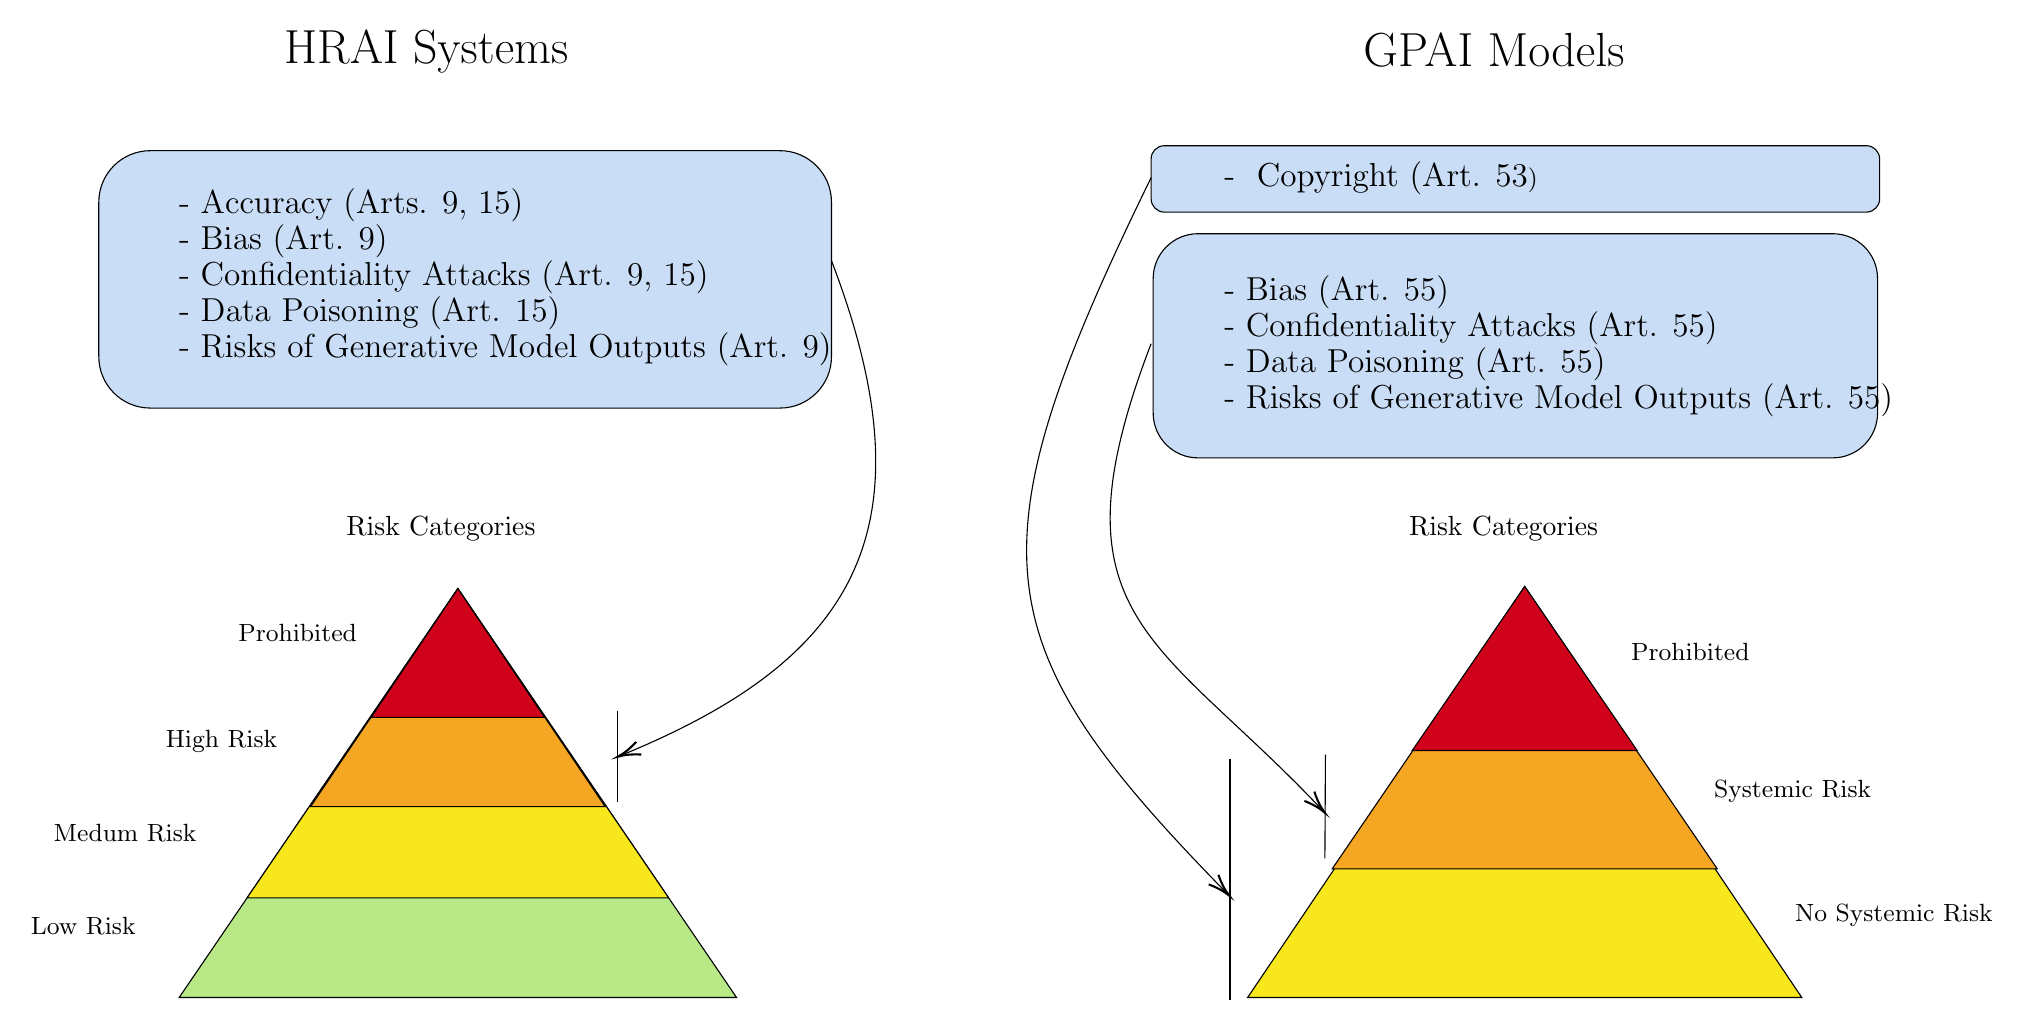
\begin{tikzpicture}[x=0.75pt,y=0.75pt,yscale=-1,xscale=1]
%uncomment if require: \path (0,592); %set diagram left start at 0, and has height of 592

%Shape: Triangle [id:dp5428005874858406] 
\draw  [fill={rgb, 255:red, 184; green, 233; blue, 134 }  ,fill opacity=1 ] (234,341) -- (368.28,538) -- (99.72,538) -- cycle ;
%Shape: Triangle [id:dp3047849031551493] 
\draw  [fill={rgb, 255:red, 248; green, 231; blue, 28 }  ,fill opacity=1 ] (748,340) -- (881.5,538) -- (614.5,538) -- cycle ;
%Shape: Triangle [id:dp0818620622382471] 
\draw  [fill={rgb, 255:red, 245; green, 166; blue, 35 }  ,fill opacity=1 ] (748,340) -- (840.75,476) -- (655.25,476) -- cycle ;
%Shape: Triangle [id:dp7631457704181537] 
\draw  [fill={rgb, 255:red, 208; green, 2; blue, 27 }  ,fill opacity=1 ] (748,340) -- (802.19,419) -- (693.81,419) -- cycle ;
%Shape: Triangle [id:dp7055596435513258] 
\draw  [fill={rgb, 255:red, 248; green, 231; blue, 28 }  ,fill opacity=1 ] (234,341) -- (335.56,490) -- (132.44,490) -- cycle ;
%Shape: Triangle [id:dp9202964178531197] 
\draw  [fill={rgb, 255:red, 245; green, 166; blue, 35 }  ,fill opacity=1 ] (234,341) -- (304.94,446) -- (163.06,446) -- cycle ;
%Shape: Triangle [id:dp09535399425331859] 
\draw  [fill={rgb, 255:red, 208; green, 2; blue, 27 }  ,fill opacity=1 ] (234,341) -- (275.77,403) -- (192.23,403) -- cycle ;
%Rounded Rect [id:dp25406852669435454] 
\draw  [fill={rgb, 255:red, 201; green, 221; blue, 246 }  ,fill opacity=1 ] (61,154.8) .. controls (61,141.1) and (72.1,130) .. (85.8,130) -- (389.2,130) .. controls (402.9,130) and (414,141.1) .. (414,154.8) -- (414,229.2) .. controls (414,242.9) and (402.9,254) .. (389.2,254) -- (85.8,254) .. controls (72.1,254) and (61,242.9) .. (61,229.2) -- cycle ;
%Rounded Rect [id:dp6638236112064699] 
\draw  [fill={rgb, 255:red, 201; green, 221; blue, 246 }  ,fill opacity=1 ] (569,191.6) .. controls (569,179.67) and (578.67,170) .. (590.6,170) -- (896.4,170) .. controls (908.33,170) and (918,179.67) .. (918,191.6) -- (918,256.4) .. controls (918,268.33) and (908.33,278) .. (896.4,278) -- (590.6,278) .. controls (578.67,278) and (569,268.33) .. (569,256.4) -- cycle ;
%Curve Lines [id:da6560168607616261] 
\draw    (414,183) .. controls (464.75,315.34) and (422.43,376.39) .. (312.66,421.32) ;
\draw [shift={(311,422)}, rotate = 337.93] [color={rgb, 255:red, 0; green, 0; blue, 0 }  ][line width=0.75]    (10.93,-3.29) .. controls (6.95,-1.4) and (3.31,-0.3) .. (0,0) .. controls (3.31,0.3) and (6.95,1.4) .. (10.93,3.29)   ;
%Straight Lines [id:da5242356218911126] 
\draw    (311,400) -- (311,444) ;
%Rounded Rect [id:dp6795269102209953] 
\draw  [fill={rgb, 255:red, 201; green, 221; blue, 246 }  ,fill opacity=1 ] (568,134) .. controls (568,130.47) and (570.87,127.6) .. (574.4,127.6) -- (912.6,127.6) .. controls (916.13,127.6) and (919,130.47) .. (919,134) -- (919,153.2) .. controls (919,156.73) and (916.13,159.6) .. (912.6,159.6) -- (574.4,159.6) .. controls (570.87,159.6) and (568,156.73) .. (568,153.2) -- cycle ;
%Straight Lines [id:da5998648988158835] 
\draw    (606,423) -- (606,539) ;
%Curve Lines [id:da489843699645353] 
\draw    (568,223) .. controls (517.26,355.34) and (571.45,363.92) .. (650.54,447.73) ;
\draw [shift={(651.73,449)}, rotate = 226.83] [color={rgb, 255:red, 0; green, 0; blue, 0 }  ][line width=0.75]    (10.93,-3.29) .. controls (6.95,-1.4) and (3.31,-0.3) .. (0,0) .. controls (3.31,0.3) and (6.95,1.4) .. (10.93,3.29)   ;
%Straight Lines [id:da4800745204547854] 
\draw    (652,421) -- (651.73,471) ;
%Curve Lines [id:da31844169520160337] 
\draw    (568,143) .. controls (479,325) and (487,368) .. (605.73,489) ;
\draw [shift={(605.73,489)}, rotate = 225.54] [color={rgb, 255:red, 0; green, 0; blue, 0 }  ][line width=0.75]    (10.93,-3.29) .. controls (6.95,-1.4) and (3.31,-0.3) .. (0,0) .. controls (3.31,0.3) and (6.95,1.4) .. (10.93,3.29)   ;

% Text Node
\draw (691,305) node [anchor=north west][inner sep=0.75pt]  [font=\normalsize] [align=left] {Risk Categories};
% Text Node
\draw (798,366) node [anchor=north west][inner sep=0.75pt]  [font=\small] [align=left] {Prohibited};
% Text Node
\draw (838,432) node [anchor=north west][inner sep=0.75pt]  [font=\small] [align=left] {Systemic Risk};
% Text Node
\draw (877,492) node [anchor=north west][inner sep=0.75pt]  [font=\small] [align=left] {No Systemic Risk};
% Text Node
\draw (179,305) node [anchor=north west][inner sep=0.75pt]  [font=\normalsize] [align=left] {Risk Categories};
% Text Node
\draw (127,357) node [anchor=north west][inner sep=0.75pt]  [font=\small] [align=left] {Prohibited};
% Text Node
\draw (92,408) node [anchor=north west][inner sep=0.75pt]  [font=\small] [align=left] {High Risk};
% Text Node
\draw (27,498) node [anchor=north west][inner sep=0.75pt]  [font=\small] [align=left] {Low Risk};
% Text Node
\draw (38,453) node [anchor=north west][inner sep=0.75pt]  [font=\small] [align=left] {Medum Risk};
% Text Node
\draw (98.4,147) node [anchor=north west][inner sep=0.75pt]  [font=\scriptsize] [align=left] {{\large - Accuracy (Arts. 9, 15)}\\{\large - Bias (Art. 9)}\\{\large - Confidentiality Attacks (Art. 9, 15)}\\{\large - Data Poisoning (Art. 15)}\\{\large - Risks of Generative Model Outputs (Art. 9)}};
% Text Node
\draw (602,189) node [anchor=north west][inner sep=0.75pt]  [font=\scriptsize] [align=left] {{\large - Bias (Art. 55)}\\{\large - Confidentiality Attacks (Art. 55)}\\{\large - Data Poisoning (Art. 55)}\\{\large - Risks of Generative Model Outputs (Art. 55)}};
% Text Node
\draw (149,71) node [anchor=north west][inner sep=0.75pt]  [font=\LARGE] [align=left] {HRAI Systems};
% Text Node
\draw (669,72) node [anchor=north west][inner sep=0.75pt]  [font=\LARGE] [align=left] {GPAI Models};
% Text Node
\draw (602.03,134) node [anchor=north west][inner sep=0.75pt]  [font=\scriptsize] [align=left] {{\large - \ Copyright (Art. 53}{\small )}};


\end{tikzpicture}

}

\end{center}
\caption{\textit{\textbf{AIA Uses Cases for Machine Unlearning.}}\label{fig:pyramids}}
\end{figure*}

 % In the meantime, we explore the application of MU to aid compliance with six system- and model-centered AIA requirements: (1) risk mitigation of risks to health and safety in AI models (2) 
 
 % Meanwhile, MU is a process for altering the behavior of an already-trained model (so that it behaves the same as a model that was not trained on the forget set) \cite{Xu_2024}. Where altering a model's behavior in this manner helps it (or the AI system it inhabits) satisfy the decreed criteria, MU's potential to aid compliance seems straightforward from a legal perspective (and the discussion then becomes one about technical feasibility). We argue this is the case for the AIA provisions requiring AI systems and/or GPAI models to mitigate certain risks \citep[Arts. 9, 55]{european_union_ai_act_2024}, to achieve accuracy and cybersecurity \citep[Art. 15]{european_union_ai_act_2024}, or to comply with EU copyright law \citep[Art. 53]{european_union_ai_act_2024}. 

 

\subsection{Accuracy}
\label{sssec:accuracy}

At least two AIA provisions may compel HRAI systems providers towards higher levels of accuracy. First (and most direct), HRAI systems must achieve a level of accuracy appropriate to their intended use and the SOTA \citep[Art. 15.1; Rec. 74]{european_union_ai_act_2024}. Second, HRAI systems' risk management must include measures to mitigate or eliminate risks to health and safety \citep[Art. 9]{european_union_ai_act_2024}, which could stem from low accuracy in domains like medicine \citep{jongsma2024why, james, Heaven2021}. For these requirements, MU can boost HRAI system's accuracy by removing the problematic data from the model. 

Importantly, the accuracy use case should not require privacy guarantees on the unlearned data \citep{goel2023adversarialevaluationsinexactmachine}. Rather, because the goal is strictly to boost accuracy to the level deemed appropriate  \citep[Art. 15]{european_union_ai_act_2024} or until the overall residual risk to health and safety posed by the inaccuracy is judged to be ''acceptable'' \citep[Art. 9]{european_union_ai_act_2024}, model accuracy should be the primary benchmark for MU's efficacy. In measuring that, AI providers will presumably account for any inadvertent, counteracting degradation in accuracy caused by the MU itself \cite{LI2024100254, DBLP:conf/sp/BourtouleCCJTZL21, Xu_2024}. However, providers will have to separately measure and account for the other trade-offs of using MU, such as its increased privacy and security risks \citep{Xu_2024, carlini2022privacyonioneffectmemorization}.  

% wherever doing so can ``reasonably'' be accomplished through the development or design of the system, to the point where the ''overall residual risk'' is ''judged to be acceptable'' \citep[Art. 9]{european_union_ai_act_2024}. 

% Even when limiting the definition of health and safety to physical safety, we can identify at least two scenarios where MU can serve as a ``post-training risk mitigation mechanism'' \citep{liu_unlearning_2023} that can help reduce, if not eliminate, the risks that problematic training data points can pose to health and safety. The first is where those problematic training data points --- e.g, mislabeled data points and outliers --- are leading to poor model performance that. 

% For example, incorrect labels in a training set may lead to model "confusion" and misclassification \cite{kurmanji2023unboundedmachineunlearning}. In the medical domain, misclassification can lead to patient harm and even "fatal outcomes" \citep{10.1001/jamadermatol.2023.5550}, including during diagnosis \cite{CHOWDHURY2024100297, PIRI201815, doi:10.4258/hir.2023.29.2.120} or triage \citep{saria2018better}. Because MU may help reduce confusion if the mislabeled examples are placed in the forget set \cite{kurmanji2023unboundedmachineunlearning, goel2023adversarialevaluationsinexactmachine}, we can logically conclude that MU, at least when it comes to incorrect labels in a training set, represents a viable mitigation for the risks to health and safety and, therefore, a path towards compliance with \citep[Art. 9]{european_union_ai_act_2024}. 

% \begin{tcolorbox}[colback=gray!10,colframe=black!50,title=State-of-the-Art]
\textbf{Current SOTA} Both exact or approximate unlearning theoretically offer paths towards improving model accuracy by forgetting mislabeled \citep{goel2023adversarialevaluationsinexactmachine,SUGIURA20242024DAT0002, 10.1145/3196494.3196517, chen2023unlearnwantforgetefficient, DBLP:conf/fgr/GundogduUU24}, out-of-date and outlier training data points \citep{kurmanji2023machineunlearninglearneddatabases, xu2024machineunlearningtraditionalmodels, Xu_2024, neel2024machineunlearning}, or, potentially, removing noise from medical data \citep{prelovznik2024improvingBrainMRI, dinsdale2020unlearningScannerBias}. The largest hurdle for this use case might be identifying all of the data points that are leading to inaccuracy (e.g., the mislabeled examples), which can be difficult \citep{goel2024correctivemachineunlearning}. However, for this use case, it may be good enough to identify only a subset of these examples --- so long as accuracy is boosted to levels deemed ''appropriate'' in light of the intended purpose as well as the SOTA \citep[Art. 15.1; Rec. 74]{european_union_ai_act_2024}. MU based on subset forget sets have shown success in boosting accuracy. However, other studies have suggested that you need all of polluted data, not just some of this, or it might backfire \citep{goel2024correctivemachineunlearning}. 
%For example, \citet{goel2024correctivemachineunlearning} demonstrate that the Selective Synaptic Dampening (SSD) MU technique \citep{foster2023fastmachineunlearningretraining} is able to neutralize mislabeled samples's effect on accuracy with just 10\% of mislabelled data identified. That said, SSD also fails (and, in fact, lowers overall accuracy) for the ''interclass confusion'' scenario (where sample labels samples are in correct between two classes)\citep{goel2024correctivemachineunlearning}.
%Evaluating MU success is application dependent. What's interesting here is that we probably don't need formal guarantees of unlearning the forget set here. We would probably want to see that accuracy is going up (or confusion down, etc.)
% \end{tcolorbox}
It is also important to note that evaluating unlearning success is application dependent. And, that, approximate unlearning should not be expected to yield higher accuracy than exact retraining without the low-quality data. 

\begin{tcolorbox}[colback=green!10,colframe=black!50,title=Key Points]
\begin{itemize}[leftmargin=0pt]
    \item Multiple AIA requirements may benefit from MU
    \item Theoretical guarantees may not be needed 
    \item Evaluation measure is application-dependent
\end{itemize}
\end{tcolorbox}

\vspace{1em}

\begin{tcolorbox}[colback=red!10,colframe=black!50,title=Open Problems]
\begin{itemize}[leftmargin=0pt]
    \item Lack of reliable methods for identifying problematic data to unlearn
    \item Lack of controllability over trade-offs
\end{itemize}
\end{tcolorbox}


% \subsubsection{MU to mitigate bias in HRAI systems and GPAI models with systemic risk} 
\vspace{1em}
\subsection{Bias} 

Providers of both HRAI systems and GPAI models with systemic risk may be obliged to mitigate model bias. The former must take measures to mitigate or eliminate risks to fundamental rights, which includes the right to non-discrimination \citep[Arts. 9]{european_union_ai_act_2024}). The latter must take measures to mitigate their models' systemic risk \citep[Art. 55]{european_union_ai_act_2024}, which includes the risk of large-scale discrimination \cite{gpai_code_2024}. Bias can occur because unrepresentative or incomplete data leads to model outputs that do not perform fairly on different groups or, in the case of generative models, produce stereotyped or otherwise discriminatory outputs \citep{sci6010003}. In all these cases, MU can ostensibly help forget the data points or patterns in the training set causing the bias \citep{pedregosa2023machineunlearning, neel2024machineunlearning, sai2024machineunlearning, keskpaik2024machine, chen2023unlearnwantforgetefficient, lucki2024adversarialperspectivemachineunlearning}. An important limiting factor on this use case is that training data that is not there to begin with cannot be forgotten; if the bias is due to a data \textit{deficit}, MU will not help. Because the goal here is to reduce or eradicate bias, success should ultimately be measured using traditional bias metrics like the difference in performance on various subgroups \citep{dealcala2023measuringbiasaimodels} or, in the case of generative models, the propensity for biased outputs as measured with benchmarks \citep{parrish2022bbqhandbuiltbiasbenchmark}.

% \begin{tcolorbox}[colback=gray!10,colframe=black!50,title=State-of-the-Art]
\textbf{Current SOTA}
While debiasing ML models was studied even before MU \citep{zemel2013learningfairreps}, both exact \citep{DBLP:journals/corr/abs-2405-14020}) and approximate \citep{chen2023fastmodeldebiasmachine, DBLP:conf/aistats/OesterlingMCL24, DBLP:journals/corr/abs-2405-14020}) MU have been used to mitigate model bias.
In the debiasing literature, solutions include \textit{pre-processing}, \textit{in-processing}, and \textit{post-processing} methods \citep{mehrabi2021fairnesssurvey}. MU, can mainly be considered as a post-processing method for debiasing. However, it is difficult to draw a separating line between debiasing and MU methods. MU works usually re-use some of the evaluation metrics in the debiasing literature, however, how to evaluate bias is, generally, considered an ``open problem'' \citep{reuel2024openproblemstechnicalai}. In order to preserve accuracy by not forgetting data points holistically, \citep{xu2024dontforgetmuchmachine} use MU to forget only those the features that lead to bias.

\begin{tcolorbox}[colback=green!10,colframe=black!50,title=Key Points]
\begin{itemize}[leftmargin=0pt]
    \item MU may assist compliance with multiple bias-related AIA requirements
    \item MU is only subtractive and never additive, limiting its application to this use case
        \item De-biasing solutions are not limited to MU
\end{itemize}
\end{tcolorbox}


\begin{tcolorbox}[colback=red!10,colframe=black!50,title=Open Problems]
\begin{itemize}[leftmargin=0pt]
    \item Lack of methods for identifying bias counterfactuals 
    \item  Lack of controllability over trade-offs
    \item Difficulty of guaranteeing full unlearning of biases, due to generalization
\end{itemize}
\end{tcolorbox}

% In multiple places, the AIA requires risks that have been identified to be mitigated \citep[Arts. 9.3, 55(a-b)]{european_union_ai_act_2024}. When it comes to HRAI systems, these risks include those to health and safety (including bias) and those to fundamental rights (including the right to data protection and the right to non-discrimination) \citep[Art. 9]{european_union_ai_act_2024}. When it comes to GPAI models, these risks include systemic risks \citep[Art. 55(a-b)]{european_union_ai_act_2024}. Where these risks owe to ``something undesirable'' in the training data, we know, at least as a technical matter, that MU can hypothetically serve as an effective (and economic) that reduces the relevant risk in the trained model (or, by extension, the AI system it inhabits) . 

% But does this mitigation meet the requirements of the law?
% Until further clarification by lawmakers or standard-setters, at least where the risk-causing qualities of the data do not independently violate requirements of the AIA, there is no reason to think that MU, when effective, cannot fulfill the risk mitigation requirements of \citep[Arts. 9.3, 55(a-b)]{european_union_ai_act_2024}.\footnote{Note that the same might be said of other ``post-training risk mitigation and defense mechanism[s]'' like alignment fine-tuning and content filters \citep{liu_unlearning_2023}.} Where the risk-causing qualities of the data \textit{do} independently violate requirements of the AIA (notably, those of Article 10), the picture could be more complicated. Are all downstream models the ``poisoned fruit'' of the non-compliant data and therefore irredeemably non-compliant themselves, regardless of any post-training risk mitigation techniques applied to them? Though we assume for the remainder of this section that this is not the case, it is a point that we ask legislators to clarify.
 % that can ``correct the impact of [the] bad data'' \citep{liu_unlearning_2023} and assist compliance with the relevant Act provision. 
% \subsubsection{MU to defend against confidentiality attacks on HRAI systems and GPAI models with systemic risk} 
\subsection{Confidentiality attacks} 
\vspace{-0.2cm}
The AIA requires providers of both HRAI systems and GPAI models with systemic risk to resolve and control for confidentiality attacks. Providers of HRAI systems must ensure their systems achieve an ``appropriate level'' of cybersecurity given the intended use and the SOTA, including by taking technical measures to prevent, detect, respond to, resolve and control for confidentiality attacks \citep[Art. 15.5; Rec. 74]{european_union_ai_act_2024}. Meanwhile, providers of GPAI models with systemic risk must ensure those models reflect ``an adequate level of cybersecurity'' \citep[Art. 55.d]{european_union_ai_act_2024}, which presumably also includes defending against confidentiality attacks. While the AIA does not define confidentiality attacks, we take them to include any attacks, including data reconstruction and membership inference attacks, that cause a model to reveal confidential details about its training such as data points or membership \citep{vassilev2023adversarial, CLTC2024adversarial}. This may include confidential training data memorized by generative models \citet{cooper2024machineunlearningdoesntthink, gu2024secondorderinformationmattersrevisiting, lucki2024adversarialperspectivemachineunlearning}. Where such attacks occur --- or where there is reason to think they might --- MU can ostensibly help defend against them by forgetting the confidential information vulnerable to attack \citep{hine_supporting_2024, neel2024machineunlearning, carlini2022privacyonioneffectmemorization, math12244001, xu2024machineunlearningtraditionalmodels, reuel2024openproblemstechnicalai, barez2025openproblemsmachineunlearning}.\footnote{We note that another, better solution to this problem exists: training with differential privacy (DP) \citep{Protivash_Durrell_Kifer_Ding_Zhang_2024}. Training a model with DP provides guarantees against confidentiality attacks \citep{chen2021differential, Protivash_Durrell_Kifer_Ding_Zhang_2024}. Accordingly, the safest strategy for complying with these AIA requirements is simply training with DP. We realize that this is not always practical, of course. AI providers --- for example, those integrating open source, closed-data models like Llama \citep{touvron2023llama} into their AI systems --- may only have access to the trained model weights and, therefore, training with DP is not an option. Differently, AI providers may only realize, post-training, that their model is vulnerable to confidentiality attacks and, at that point, may not be in a position to bear the cost of retraining from scratch with DP. In these situations, approximate unlearning remains a highly relevant option for addressing these attacks.} For this use case, the measure of success should be whether confidentiality attacks succeed in the wake of the MU \cite{grimes2024goneforgottenimprovedbenchmarks}, though use case-specific metrics have been developed \citet{maini2024tofutaskfictitiousunlearning}. When it comes to this use case, there are, importantly, other viable options for protecting against confidentiality attacks, including training with DP \citep{WANG2023408, kaissis2023boundingdatareconstructionattacks}.
% \begin{tcolorbox}[colback=gray!10,colframe=black!50,title=State-of-the-Art]

\textbf{Current SOTA.} Multiple techniques for using MU to mitigate confidentiality attacks (or the closely related problem of inadvertent model leakage of personal data) have been demonstrated \citep{dhingra2024protecting, ashuach2024revsunlearningsensitiveinformation, lizzo2024unlearnefficientremovalknowledge, chen2024, Wang_2024, CaoYang2015, DBLP:conf/sp/BourtouleCCJTZL21, Borkar}.
As of today, using MU to thwart these attacks can carry sizable trade-offs. For example, unlearning some data points for the sake of protecting them from recovery by attackers can jeopardize the privacy of other data points that neighbor the ones that have been unlearned \citet{carlini2022privacyonioneffectmemorization} or even increase the risk of membership inference attacks that recover the unlearned data points \citet{Chen_2021, barez2025openproblemsmachineunlearning,kurmanji2023unboundedmachineunlearning}. Differently, approximate unlearning, when used to delete particular data points, can carry a bias trade-off \citep{zhang2023forgotten, oesterling2024fairmachineunlearningdata} and an accuracy trade-off that rises as more data is forgotten \citep{Graves_Nagisetty_Ganesh_2021, maini2024tofutaskfictitiousunlearning}. It is also important to note that current MU methods, usually fail on new emergent attacks that are devised with new assumptions \citep{zhang2024doesmureallyforgets, hu2024joggingmumemory}.

\begin{tcolorbox}[colback=green!10,colframe=black!50,title=Key Points]
\begin{itemize}[leftmargin=0pt]
    \item MU may assist compliance with multiple confidentiality attack-related AIA requirements
    \item Due to attack diversity, success should be measured on case-by-case basis
    \item DP is a strong alternative to MU for this use case
\end{itemize}
\end{tcolorbox}

\begin{tcolorbox}[colback=red!10,colframe=black!50,title=Open Problems]
\begin{itemize}[leftmargin=0pt]
    \item Difficulty of providing formal guarantees of attack susceptibility 
    \item  Difficulty of applying MU to new, emergent attacks
    \item Identifying, localizing, and measuring memorization of confidential data is itself an open problem
\end{itemize}
\end{tcolorbox}

% \subsubsection{MU to mitigate data poisoning and backdoor attacks in HRAI systems and GPAI models with systemic risk} 
\subsection{Data poisoning} 
In data poisoning, specially-crafted data points are injected into a training set to alter (e.g., degrade or bias) the behavior of the model to the benefit the attacker \citep{DBLP:conf/icml/BiggioNL12}. Backdoor attacks are a type of data poisoning where the injected data points create ``triggers'' the attacker can exploit during inference \citep{lin2021mlattackmodelsadversarial}. The AIA obligates the providers of both HRAI systems and GPAI model with systemic risk to address such attacks. HRAI system providers must ensure their systems achieve an ``appropriate level'' of  cybersecurity, including via technical measures to ``prevent, detect, respond to, resolve and control for attacks trying to manipulate the training data set (data poisoning)'' \citep[Art. 15(5)]{european_union_ai_act_2024}.\footnote{HRAI system providers may additionally be compelled to address data poisoning in order to comply with those AIA provisions, discussed in \ref{sssec:accuracy}, necessitating a certain level of accuracy --- since model poisoning can degrade accuracy \citep{nawshin2024assessing}.} Providers of GPAI models with systemic risk, meanwhile, must ``ensure an adequate level of cybersecurity'' in their models \citep[Art. 55.d]{european_union_ai_act_2024}, which presumably also includes defenses against data poisoning. Where it is known that data poisoning has (or could) occur, MU may help remove the effects of the poisoned data points on the model and, thus, help satisfy these requirements  \citep{Xu_2024, liu2024threatsattacksdefensesmachine, CaoYang2015, 10.1145/3196494.3196517, 281308}. When it comes to measuring success for this use case, because the ``primary goal is to unlearn the adverse effect due to the manipulated data,'' the ideal benchmark would seem to be whether those adverse effects --- be they vulnerability to backdoor triggers, bias, or lower accuracy --- are eliminated or reduced \citep{goel2024correctivemachineunlearning}. For example, \citet{goel2024correctivemachineunlearning} measure MU efficacy based on whether proper accuracy on backdoor triggers is restored.

% \begin{tcolorbox}[colback=gray!10,colframe=black!50,title=State-of-the-Art]
\textbf{Current SOTA} Though some work has demonstrated MU can succeed for this use case \citep{warnecke2023machineunlearningfeatureslabels, schoepf2024potionpoisonunlearning} other works question the effectiveness of using MU to address data poisoning or backdoor attacks specifically \citep{8685687, 10.1007/978-3-030-58951-6_24, pawelczyk2024machineunlearningfailsremove, xu2024machineunlearningtraditionalmodels}). As always, identifying the full forget set (here, the poisoned samples) remains challenging \citep{goel2024correctivemachineunlearning}. Some methods, moreover, can have a significant accuracy trade-off on this use case \citep{pawelczyk2024machineunlearningfailsremove}. Such trade-offs can be particularly difficult as poisoned data overlaps with the clean data and, in most cases, they are even visually indistinguishable from each other.  

\begin{tcolorbox}[colback=green!10,colframe=black!50,title=Key Points]
\begin{itemize}[leftmargin=0pt]
    \item MU may assist compliance with multiple data poisoning-related AIA requirements
    \item A proper benchmark should measure the elimination of adverse effects
\end{itemize}
\end{tcolorbox}

\begin{tcolorbox}[colback=red!10,colframe=black!50,title=Open Problems]
\begin{itemize}[leftmargin=0pt]
    \item Finding contaminated data at scale is challenging 
    \item Unlearning the backdoor pattern without hurting unaffected data is challenging 
        \item Current MU methods mostly fail on data poisoning use case
\end{itemize}


\end{tcolorbox}


% \subsubsection{MU to mitigate the risks to health, safety, and fundamental rights and systemic risk posed by the generative outputs of HRAI systems and GPAI models with systemic risk} 
\subsection{Other risks of generative outputs} 

Generative model outputs may pose risks to health, safety, and human rights or pose systemic risk that the providers of HRAI systems and GPA models, respectively, must mitigate. For example, HRAI systems' risk management systems must include measures to mitigate or eliminate risks that the system poses to health, safety, and fundamental rights \citep[Art. 9]{european_union_ai_act_2024}. Generative model outputs may pose risks to health and safety, for example by issuing bad medical advice \citep{wu2024generating, Han2024}); likewise, generative model outputs may pose a risk to the fundamental right of non-discrimination, for example by producing stereotyping outputs \citep{nicoletti2023humans}. When it comes to GPAI models with systemic risk, providers of such models must mitigate that systemic risk \citep[Art. 55]{european_union_ai_act_2024}, which could be brought on by generative model outputs  that display offensive cyber capabilities, knowledge of CBRN, and more \cite{gpai_code_2024, nist2024trustworthy}. In all of these cases, MU may help mitigate the non-compliant outputs by unlearning the data points or even the concepts in the training set that are causing them \cite{lucki2024adversarialperspectivemachineunlearning, cooper2024machineunlearningdoesntthink}. Computationally, it may offer advantages even as compared to other popular alignment techniques like reinforcement learning  \citep{yao2024largelanguagemodelunlearning}. Measuring success for this use case should arguably be ``context dependent'' \citep{yao2024largelanguagemodelunlearning}. That is, the best way to measure the MU's efficacy is to benchmark the specific behavior that we desire to repair \citep{yao2024largelanguagemodelunlearning}. This could be done using existing benchmarks unrelated to MU \cite{barez2025openproblemsmachineunlearning}. Differently, \citep{li2024wmdpbenchmarkmeasuringreducing} propose a benchmark for measuring MU of CBRN knowledge. That being said, approaches that examine the model parameters for remnants of the unlearned concepts have also been proposed \citep{hong2024intrinsicevaluationunlearningusing}.

% \begin{tcolorbox}[colback=gray!10,colframe=black!50,title=State-of-the-Art]
\textbf{Current SOTA}
Multiple works use MU to curb undesirable generative model outputs  \cite{omkar, yu-etal-2023-unlearning, WEI2025104103, fore2024unlearningclimatemisinformationlarge}. However, the task is difficult, without agreed-upon best practices \citep{cooper2024machineunlearningdoesntthink}. Broad concepts like non-discrimination tend to go beyond individual data points, to latent information which is not easily embodied as a discrete forget set \cite{cooper2024machineunlearningdoesntthink, liu_unlearning_2023}. Even if data points that are intrinsically harmful (e.g., the molecular structure of a biological weapon) are removed, models may still assemble dangerous outputs from latent information in the rest of the dataset \citep{cooper2024machineunlearningdoesntthink, intl_ai_safety_2025}. Trying to remove that latent knowledge can risk model utility \cite{cooper2024machineunlearningdoesntthink}. As a separate but related issue, AI systems in these scenarios may be dual-use, where the appropriateness of outputs depends on downstream context; this, too, makes identifying the forget set difficult and increases the likelihood of a utility trade-off as the model forgets useful knowledge alongside undesirable knowledge \cite{cooper2024machineunlearningdoesntthink, shi2024musemachineunlearningsixway, reuel2024openproblemstechnicalai}. All of these issues, in turn, make it difficult if not impossible to specify formal guarantees on the MU \citep{liu_unlearning_2023}. 
% \end{tcolorbox}

\begin{tcolorbox}[colback=green!10,colframe=black!50,title=Key Points]
\begin{itemize}[leftmargin=0pt]
    \item MU may assist compliance with multiple AIA requirements related to generative outputs
\end{itemize}
\end{tcolorbox}

\begin{tcolorbox}[colback=red!10,colframe=black!50,title=Open Problems]
\begin{itemize}[leftmargin=0pt]
    \item Defining the forget set when what we seek to forget is conceptual  
    % \citep{cooper2024machineunlearningdoesntthink}
    \item Difficulty of guaranteeing full unlearning of undesirable behaviors, due to generalization
        % \citep{cooper2024machineunlearningdoesntthink}
            \item Mitigating the forgetting of useful knowledge alongside undesirable knowledge 
            % \citep{reuel2024openproblemstechnicalai}
\end{itemize}
\end{tcolorbox}

% \subsubsection{MU to comply with copyright law in GPAI models}
\subsection{Copyright}
All GPAI model providers must have a policy for complying with EU law on ``copyright and related rights'' \citep[Art. 53.c]{european_union_ai_act_2024}. Among other things, this policy must honor the TDM opt-outs of rightsholders \citep[Art. 53.c; Rec. 105]{european_union_ai_act_2024}, which is often a feature of AI training \citep{Rosati_2024, kneschke2024laion}. When it comes to AI and copyright law, a distinction is sometimes made between the ``input'' (training) phase and the ``output'' (inference) phase of the AI life cycle \citep{Rosati_2024, quintais2024generative}. At this point in time, the primary compliance risk during the input phase seems to be that an AI training set could include data points that violate TDM opt-outs. When this happens, we assume that using MU to remove the opt-out data points from the trained model does not cure the violation, since the violation occurred at the moment the opt-out data was used for training.\footnote{This topic --- whether MU can assuage the violation of TDM opt-outs or whether the proverbial ship has sailed --- is another that could use clarification from EU lawmakers.\label{footnote7}} That said, MU may still represent a valuable component of a copyright-compliance policy by helping prevent, at the ``output'' phase, further violations of copyright law when the opt-out data points --- or any other copyright-protected data points in the training set --- are reproduced to some degree in model outputs \citep{Rosati_2024}. This is a real risk with generative models, which often memorize training data \citep{cooper2024files, carlini2023extractingtrainingdatadiffusion}. When MU is applied to this use case, we want to measure success by tracking how likely the model is to generate works that are sufficiently similar to the copyrighted works. For example, we might rely on existing benchmarks that measure the tendency of models to produce copyrighted materials \citep{liu2024shieldevaluationdefensestrategies, chen2024copybenchmeasuringliteralnonliteral}. Differently, \citet{ma2024datasetbenchmarkcopyrightinfringement} produce a benchmark for the success of MU in the copyright context.

% \begin{tcolorbox}[colback=gray!10,colframe=black!50,title=State-of-the-Art]
\textbf{Current SOTA}
\citet{wu2024unlearningconceptsdiffusionmodel} unlearn copyrighted works from diffusion models.
At first glance, exact MU would seem to provide a guarantee that copyrighted works in the training set will not be reproduced in outputs \cite{liu_unlearning_2023}. But the fact is that retraining from scratch without the copyrighted data points may not be a bulletproof solution for preventing copyright infringement in outputs because substantially similar representations of copyrighted ``expressions'' (e.g., images of characters like Spiderman) could still appear in outputs based on how the model generalizes from the latent information extracted from the rest of the training set \citet{cooper2024machineunlearningdoesntthink}. For the same reason, approximate unlearning aimed at removing the influence of the copyright data points on the model, on top of being hard to prove \citep{liu_unlearning_2023},  also cannot ensure that copyrights are not infringed by outputs. In general, the SOTA of approximate unlearning has been deemed ``insufficient'' for the copyright use case, which may be why practitioners currently lean towards pre- and post-processing tools like prompting and moderation to bring AI into compliance with these laws \citep{liu_unlearning_2023, shumailov2024ununlearningunlearningsufficientcontent}.
\citep{dou2024avoidingcopyrightinfringementlarge} ``unlearn'' copyrighted materials in LLM pre-training datasets by identifying and removing specific weight updates in the model’s parameters that correspond to copyrighted content, evaluating their method by measuring the similarities between the model’s outputs
and the original content.
The task of measuring whether substantially similar outputs are being produced is quite challenging \citep{cooper2024machineunlearningdoesntthink}.


\begin{tcolorbox}[colback=green!10,colframe=black!50,title=Key Points]
\begin{itemize}[leftmargin=0pt]
    \item MU does not help with TDM opt-out violations; the damage is already done
    \item MU may, however, help with downstream copyright violations in outputs
    \item To avoid malicious unlearning, TDM opt-outs will have to be verified 
\end{itemize}
\end{tcolorbox}

\begin{tcolorbox}[colback=red!10,colframe=black!50,title=Open Problems]
\begin{itemize}[leftmargin=0pt]
    \item Difficulty in identifying copyright-infringing works in a dataset 
    % \citep{cooper2024machineunlearningdoesntthink}
    \item Difficulty of verifying whether model output is due to copyrighted content or generalization 
        \item Localizing and measuring memorization of copyrighted data is itself an open problem
    % \citep{liu2024threatsattacksdefensesmachine}.
\end{itemize}
\end{tcolorbox}

 


\section{Conclusion}
\label{Conclusion}
Despite its many challenges, MU has great potential as a tool for AIA compliance. Because contemporary AI regulations tend to feature recurring principles \citep{doi:10.1080/13510347.2023.2196068, DIAZRODRIGUEZ2023101896}, this likely means that MU has great potential as a tool for compliance with other AI regulations too. To realize this potential, AI researchers should help solve the (sometimes critical) open technical problems logged by this position paper. Among other things, this includes work on identifying forget set data points, on resolving the privacy and performance trade-offs of MU, and on resolving the particular challenges to these use cases that generative model outputs present. While researchers investigate these open problems, lawmakers can support them by explicitly endorsing MU as a compliance tool for AI regulation requirements and, more acutely, resolving some of the particular legal ambiguities we have flagged in this position paper (\ref{footnote2},\ref{footnote7}). Working collaboratively, we can all help unlock MU’s potential to assist compliance with the AI regulation and, by extension, help safeguard the important social values these regulations encode. 

% \section*{Impact Statement}

% In essence, this position paper suggests research directions that will help MU evolve into a better tool for assisting AI regulation compliance. Because these AI regulations tend to protect important ethical and societal values around health and safety, non-discrimination, and more, we believe the impact of this paper, in striving to advance AI regulation compliance through MU, will ultimately be the advancement of those important values as well.

\section*{Acknowledgements}
\textit{Funding}. We wish to acknowledge the Google Academic Research Awards for their support.

% In the unusual situation where you want a paper to appear in the
% references without citing it in the main text, use \nocite

  
\bibliography{example_paper}
\bibliographystyle{icml2025}


%%%%%%%%%%%%%%%%%%%%%%%%%%%%%%%%%%%%%%%%%%%%%%%%%%%%%%%%%%%%%%%%%%%%%%%%%%%%%%%
%%%%%%%%%%%%%%%%%%%%%%%%%%%%%%%%%%%%%%%%%%%%%%%%%%%%%%%%%%%%%%%%%%%%%%%%%%%%%%%
% APPENDIX
%%%%%%%%%%%%%%%%%%%%%%%%%%%%%%%%%%%%%%%%%%%%%%%%%%%%%%%%%%%%%%%%%%%%%%%%%%%%%%%
%%%%%%%%%%%%%%%%%%%%%%%%%%%%%%%%%%%%%%%%%%%%%%%%%%%%%%%%%%%%%%%%%%%%%%%%%%%%%%%
% \newpage
% \appendix
% \onecolumn
% \section{Appendix: End notes.}

% \theendnotes
%%%%%%%%%%%%%%%%%%%%%%%%%%%%%%%%%%%%%%%%%%%%%%%%%%%%%%%%%%%%%%%%%%%%%%%%%%%%%%%
%%%%%%%%%%%%%%%%%%%%%%%%%%%%%%%%%%%%%%%%%%%%%%%%%%%%%%%%%%%%%%%%%%%%%%%%%%%%%%%


\end{document}


% This document was modified from the file originally made available by
% Pat Langley and Andrea Danyluk for ICML-2K. This version was created
% by Iain Murray in 2018, and modified by Alexandre Bouchard in
% 2019 and 2021 and by Csaba Szepesvari, Gang Niu and Sivan Sabato in 2022.
% Modified again in 2023 and 2024 by Sivan Sabato and Jonathan Scarlett.
% Previous contributors include Dan Roy, Lise Getoor and Tobias
% Scheffer, which was slightly modified from the 2010 version by
% Thorsten Joachims & Johannes Fuernkranz, slightly modified from the
% 2009 version by Kiri Wagstaff and Sam Roweis's 2008 version, which is
% slightly modified from Prasad Tadepalli's 2007 version which is a
% lightly changed version of the previous year's version by Andrew
% Moore, which was in turn edited from those of Kristian Kersting and
% Codrina Lauth. Alex Smola contributed to the algorithmic style files.
